% Final project report. Compile: latexmk -pdf FINAL_REPORT.tex   (tables: python make_tables.py)
\documentclass[11pt,a4paper]{article}
\usepackage[margin=2.2cm]{geometry}
\usepackage{graphicx,booktabs,float,caption,subcaption,xcolor,pifont,enumitem,amsmath}
\usepackage{tikz,array}
\usepackage[most]{tcolorbox}
\usepackage{adjustbox}
\usepackage[colorlinks=true,linkcolor=blue!50!black,urlcolor=blue!50!black,citecolor=blue!50!black]{hyperref}
\graphicspath{{../Logos/}{../figures/}{../figures/story/}{../figures/report/}{../figures/app/}}
\definecolor{vn}{HTML}{C0392B}
\setlist{itemsep=2pt,topsep=3pt}
\captionsetup{font=small,labelfont=bf}
\newtcolorbox{summary}[1][Summary]{colback=blue!3,colframe=blue!45!black,fonttitle=\bfseries,title=#1,
  boxrule=0.6pt,arc=2pt,left=6pt,right=6pt,top=4pt,bottom=4pt}
\newcommand{\var}[1]{\texttt{#1}}
\newcommand{\tab}[1]{\begin{adjustbox}{max width=\textwidth}\input{tables/#1.tex}\end{adjustbox}}
\setlength{\parskip}{4pt}\setlength{\parindent}{0pt}

\usepackage[section]{placeins}   % floats never drift into the next section
\renewcommand{\topfraction}{0.9}\renewcommand{\bottomfraction}{0.8}\renewcommand{\textfraction}{0.07}
\renewcommand{\floatpagefraction}{0.75}\setcounter{topnumber}{3}\setcounter{totalnumber}{5}
\newcommand{\frontsection}[1]{\section*{#1}\addcontentsline{toc}{section}{#1}}

\begin{document}

% ------------------------------------------------------------------ cover
\begin{titlepage}
\centering
\setlength{\parskip}{0pt}
\vspace*{0.45cm}
\begin{tikzpicture}[remember picture,overlay]
\draw[line width=2.2pt] ([xshift=1.2cm,yshift=-1.2cm]current page.north west) rectangle ([xshift=-1.2cm,yshift=1.2cm]current page.south east);
\draw[line width=0.5pt] ([xshift=1.55cm,yshift=-1.55cm]current page.north west) rectangle ([xshift=-1.55cm,yshift=1.55cm]current page.south east);
\end{tikzpicture}%
{\large\bfseries VIET NAM NATIONAL UNIVERSITY HO CHI MINH CITY\par}
\vspace{0.4cm}
{\large\bfseries HO CHI MINH CITY UNIVERSITY OF TECHNOLOGY\par}
\vspace{0.4cm}
{\large\bfseries FACULTY OF COMPUTER SCIENCE AND ENGINEERING\par}
\vspace{0.5cm}

\includegraphics[width=6.3cm]{01_logobachkhoasang.png}\par
\vspace{1.0cm}
{\itshape Report of\par}
\vspace{0.3cm}
{\Large\bfseries RESEARCH TOPIC: DATA ANALYTICS\par}
\vspace{1.3cm}
{\itshape Topic:\par}
\vspace{0.3cm}
{\LARGE\bfseries DOES RICHER MEAN\\[3pt] MORE DEVELOPED?\par}
\vspace{0.3cm}
{\Large\bfseries A data-mining study of the World\\[2pt] Development Indicators, 1960--2014\par}
\vspace{1.1cm}
{\large\bfseries Lecturer:\quad Dr. Nguyen Thi Ai Thao\par}
\vspace{1.2cm}
{\renewcommand{\arraystretch}{1.6}\small
\begin{tabular}{|>{\centering\arraybackslash}p{5.6cm}|>{\centering\arraybackslash}p{4.2cm}|}
\hline
\textbf{Member} & \textbf{Student's ID} \\
\hline
Le Thi Hong Cuc & 2470882 \\
\hline
Phan Van Nguyen Khanh & 2470883 \\
\hline
Nguyen Tuong Phuc & 2470886 \\
\hline
\end{tabular}\par}
\vfill
{\large\bfseries HO CHI MINH CITY, NOVEMBER 2026\par}
\vspace{1.3cm}
\end{titlepage}

% ------------------------------------------------------------------ front matter
\pagenumbering{roman}

\frontsection{Abstract}
This report examines whether higher national income is associated with higher levels of development across health, education, demography, environment and technology. The analysis uses the Kaggle extract of the World Bank World Development Indicators (5.66 million observations, 247 economies, 1,344 indicators, 1960--2015), from which 32 indicators in six themes were selected for 214 countries. An initial exploration quantifies the size and structure of the data, the distributions of the attributes, the outliers and groups of similar countries, and the effect of missing values, which affect 44.9\,\% of the country-year cells and are not missing at random. A preprocessing pipeline covering cleaning, integration, transformation and reduction produces a country-year panel ($11{,}935 \times 32$) and a cross-country snapshot ($214 \times 32$).

Three research questions are addressed with nine experiments. First, $\sigma$- and $\beta$-convergence analyses show that health and schooling converged across countries (the cross-country coefficient of variation of life expectancy fell by 47\,\%) whereas income did not ($\beta$-convergence $r = -0.15$, $p = 0.054$); the result is robust to a balanced panel and to population weighting. Second, cross-validated models with country-grouped folds show that the logarithm of GDP per capita alone explains 51--77\,\% of the cross-country variance of five development themes (mean $R^2 = 0.63$), compared with a mean of 0.82 for the best of 19 regressors. A two-way fixed-effects model indicates that the within-country association between income and life expectancy (3.2 years per tenfold increase) is about one third of the between-country association (10.9 years). Third, unsupervised clustering reproduces the World Bank income groups for 74\,\% of countries but is not stable across algorithms (adjusted Rand index of about 0.55), which suggests that development is better described as a continuum than as discrete groups. Vietnam, used as a case study throughout, has the largest positive life-expectancy residual among 203 countries (+10.4 years) and social outcomes comparable to countries 3.5 to 14.5 times richer, but it emits 3.2 times the CO$_2$ predicted by its income. All results are reproducible from the accompanying code and are presented in an interactive web application.

\textbf{Keywords:} World Development Indicators; economic development; convergence; Preston curve; missing data; cross-validation; clustering; Vietnam.

\clearpage
\tableofcontents
\clearpage
\addcontentsline{toc}{section}{List of Figures}
\listoffigures
\bigskip
\addcontentsline{toc}{section}{List of Tables}
\listoftables

\clearpage
\frontsection{List of Abbreviations}
\begin{table}[htbp]\centering\small
\begin{tabular}{ll}
\toprule
Abbreviation & Meaning \\
\midrule
ARI & Adjusted Rand index \\
CAGR & Compound annual growth rate \\
CV & Coefficient of variation (standard deviation divided by mean) \\
EKC & Environmental Kuznets curve \\
FE & Fixed effects (panel regression) \\
GDP & Gross domestic product \\
IQR & Interquartile range \\
MAE / RMSE & Mean absolute error / root mean squared error \\
MAR / MCAR / MNAR & Missing at random / completely at random / not at random \\
OLS & Ordinary least squares \\
PCA & Principal component analysis \\
PPP & Purchasing power parity \\
$R^2$ & Coefficient of determination \\
RQ / H & Research question / hypothesis \\
SD & Standard deviation \\
WDI & World Development Indicators \\
\bottomrule
\end{tabular}
\end{table}

\clearpage
\pagenumbering{arabic}

% ================================================================== 1
\section{Introduction}\label{sec:intro}

\subsection{Background and motivation}
Gross domestic product per capita is the most widely reported summary of a country's economic position, and it is frequently used, explicitly or implicitly, as a proxy for development as a whole: the World Bank, for example, classifies economies into four groups by income alone. Development, however, is a multidimensional concept that also comprises health, education, demographic change, environmental pressure and access to technology. Whether these dimensions follow income closely, or whether countries at similar income levels achieve very different outcomes, is therefore a question of both scientific and practical interest. If income determines most of the variation, income-based classifications are an adequate shortcut; if it does not, they may mask both successes and failures that deserve attention.

The World Development Indicators (WDI) are the World Bank's principal collection of internationally comparable country statistics \cite{wdi}. Their breadth (more than a thousand indicators over five decades) makes them well suited to a data-mining study of this question, but their sparsity, heterogeneous coverage and skewed distributions also make careful exploration and preprocessing a prerequisite for any valid conclusion.

\subsection{Problem statement and research questions}
The study is organised around one overarching question:

\begin{center}\large\itshape To what extent does higher national income correspond to higher development?\end{center}

Following the descriptive, diagnostic and prescriptive levels of analytics, the overarching question is decomposed into three research questions:
\begin{description}[leftmargin=1.2cm,style=nextline]
\item[RQ1] (\emph{descriptive}) How did development indicators evolve between 1960 and 2014, and did countries become more similar over time?
\item[RQ2] (\emph{diagnostic}) How much of the cross-country variation in development outcomes is explained by income, and which countries perform substantially better or worse than their income predicts?
\item[RQ3] (\emph{prescriptive}) Do data-driven groupings of countries coincide with income-based groupings, and where does a given country, Vietnam, stand when it is compared on outcomes rather than on income?
\end{description}

From the literature reviewed in Section~\ref{sec:related} the following hypotheses are derived and tested in Section~\ref{sec:results}:
\begin{description}[leftmargin=1.2cm,style=nextline]
\item[H1] Social outcomes (health, schooling, technology) converged across countries ($\sigma$-convergence).
\item[H2] Income per capita did not converge unconditionally across countries.
\item[H3] Income alone explains the majority of the cross-country variance in each development theme.
\item[H4] The association between income and life expectancy is weaker within countries over time than between countries.
\item[H5] Clusters obtained from development outcomes reproduce the World Bank income groups.
\end{description}

\subsection{Objectives}
The project pursues four objectives, which correspond to the requirements of the assignment:
\begin{enumerate}
\item to explore the raw WDI data, describing its size and attributes, its summary statistics, its outliers and groups, and the effect of missing values on each of these (Section~\ref{sec:A});
\item to design and apply a preprocessing pipeline whose techniques are justified by the problems found during exploration (Section~\ref{sec:B});
\item to answer RQ1--RQ3 with data-mining methods (trend and convergence analysis, regression, panel models, clustering and similarity search) under an evaluation protocol that prevents information leakage (Sections~\ref{sec:method} and~\ref{sec:results});
\item to make the analysis reproducible and accessible through open code and an interactive web application (Section~\ref{sec:app}).
\end{enumerate}

\subsection{Scope}
The study uses the Kaggle release of the WDI \cite{kaggle}, which ends in 2014--2015; results therefore describe the period 1960--2014 and the income classification in force at the time. The unit of analysis is the country: medians and correlations are not weighted by population unless stated otherwise (Section~\ref{sec:conv}). Vietnam is used as a recurring case study and is highlighted in \textcolor{vn}{\textbf{red}} in every figure; its five regional comparators are China, Thailand, Indonesia, the Philippines and Malaysia. The analysis is associational; no causal effect of income is claimed (Section~\ref{sec:validity}).

\subsection{Contributions}
The contributions of this work are threefold. First, it provides a systematic audit of the WDI extract, including a quantitative assessment of how missing values bias summary statistics and correlations. Second, it measures the explanatory power of income across five development themes within a single, leakage-controlled framework (country-grouped cross-validation over 19 regressors), and complements the cross-sectional view with a within-country panel estimate. Third, it combines residual analysis, clustering and nearest-neighbour search to position an individual country on outcomes rather than on income, and tests the robustness of each result.

\subsection{Organisation of the report}
Section~\ref{sec:related} defines the key concepts and reviews related work. Section~\ref{sec:A} reports the initial data exploration and Section~\ref{sec:B} the preprocessing pipeline. Section~\ref{sec:method} describes the analytical methods and the evaluation protocol, and Section~\ref{sec:results} presents the results by research question. Section~\ref{sec:app} describes the interactive web application. Section~\ref{sec:discussion} discusses the findings, their relation to the literature and the threats to validity, and Section~\ref{sec:conclusion} concludes. The appendices list the selected indicators, the reproduction steps and the repository structure.

% ================================================================== 2
\section{Background and related work}\label{sec:related}

\subsection{Definition of terms}
\begin{description}[leftmargin=0.6cm,style=nextline]
\item[Development indicator] A country-level statistic that measures one aspect of living conditions, such as life expectancy at birth, gross secondary enrolment or internet users per 100 people. In this report indicators are grouped into six themes: economy, demography, health, education, environment and technology.
\item[Preston curve] The concave relationship between national income per capita and life expectancy, steep at low incomes and flat at high incomes, which has shifted upwards over time \cite{preston}.
\item[$\sigma$-convergence] A decrease over time in the dispersion of an indicator across countries, here measured by the coefficient of variation \cite{barro}.
\item[$\beta$-convergence] A negative relationship between the initial level of an indicator and its subsequent rate of change, meaning that countries that start lower improve faster \cite{barro}.
\item[Environmental Kuznets curve] The hypothesis that environmental pressure first rises and then falls with income, implying a turning point beyond which growth reduces emissions \cite{grossman}.
\item[Missing-data mechanisms] Values are missing completely at random (MCAR) when missingness is unrelated to any variable, at random (MAR) when it depends only on observed variables, and not at random (MNAR) when it depends on the unobserved value itself \cite{little}.
\item[Residual (performance relative to income)] The difference between a country's observed outcome and the outcome predicted from its income alone, computed out of fold so that the country does not influence its own prediction.
\end{description}

\subsection{Literature review}
\paragraph{Income and health.} Preston \cite{preston} showed that life expectancy rises steeply with national income at low levels and flattens at high levels, and that the entire curve shifts upward over time. In a later retrospective he attributed most of this shift to factors other than income, such as medical knowledge and public-health technology \cite{preston07}; Bloom and Canning \cite{bloom07} discuss why the relationship remains contested. Whether income itself causes better health is a distinct question. Using instrumental variables on cross-country time series, Pritchett and Summers \cite{pritchett} estimate a long-run income elasticity of infant and child mortality between $-0.2$ and $-0.4$ in developing countries, which supports the proposition that wealthier is healthier. Deaton \cite{deaton} reviews the evidence on health, income and inequality and cautions that raw correlations conflate several mechanisms.

\paragraph{Outcomes beyond income.} A second strand of the literature argues that income is neither necessary nor sufficient for good social outcomes. Caldwell \cite{caldwell} examined societies with unusually low mortality relative to their income, such as Sri Lanka, Kerala and Costa Rica, and attributed their performance to female education and accessible health services rather than to growth. Anand and Ravallion \cite{anand} reach a related conclusion: income matters mainly through poverty reduction and the public services it finances. These ``over-achievers'' are the countries that the residual analysis of this study is designed to detect.

\paragraph{Convergence.} A third strand asks whether poorer countries catch up. Barro and Sala-i-Martin \cite{barro} formalised the concepts of $\beta$- and $\sigma$-convergence. Mankiw, Romer and Weil \cite{mrw} found that convergence emerges only once physical and human capital are held constant (conditional convergence), and Sala-i-Martin \cite{sala06} showed that inequality between individuals worldwide fell in the 1980s and 1990s even though gaps between countries persisted.

\paragraph{Growth and the environment.} Grossman and Krueger \cite{grossman} reported an inverted-U relationship between income and several pollutants, which gave rise to the environmental Kuznets curve. Whether such a turning point exists for carbon dioxide, a global rather than local pollutant, is less clear, which motivates including the environment theme in this study.

\paragraph{Methodological background.} The data-mining process followed here, from cleaning and integration to transformation and reduction, is standard \cite{han}. The treatment of missing values follows the taxonomy of Little and Rubin \cite{little}, the panel models follow Wooldridge \cite{wooldridge}, and cluster quality is assessed with the silhouette coefficient \cite{rousseeuw} and the adjusted Rand index \cite{hubert}.

\subsection{Position of this work}
Table~\ref{tab:lit} relates the core literature to the experiments of this study. Most prior studies test one hypothesis on one or two indicators with econometric models. The present work is narrower in its causal ambition but broader in coverage: it applies a single reproducible pipeline to 32 indicators, evaluates predictive claims out of sample with country-grouped cross-validation, and adds unsupervised methods to describe a country's position beyond its income.

\begin{table}[htbp]\centering\footnotesize
\caption{Core literature and its relation to the experiments of this study.}\label{tab:lit}
\begin{tabular}{p{3.0cm}p{3.2cm}p{5.0cm}p{3.6cm}}
\toprule
Work & Approach & Key finding & Link to this study \\
\midrule
Preston 1975, 2007 \cite{preston,preston07} & Cross-country curve fitting & Concave income--life expectancy curve that shifts upward over time & Preston curve, E2.2, year effects in E2.3 \\
Pritchett \& Summers 1996 \cite{pritchett} & Instrumental variables, panel & Income reduces child mortality (elasticity $-0.2$ to $-0.4$) & Within-country slope, E2.3 \\
Caldwell 1986 \cite{caldwell}; Anand \& Ravallion 1993 \cite{anand} & Case studies; cross-country regression & Low mortality is achievable at low income through public services & Residual scorecard, E2.2 \\
Barro \& Sala-i-Martin 1992 \cite{barro} & $\beta$/$\sigma$-convergence & Unconditional income convergence is absent across countries & E1.1--E1.3 \\
Mankiw et al.\ 1992 \cite{mrw}; Sala-i-Martin 2006 \cite{sala06} & Augmented Solow model; income distribution & Convergence is conditional; individual inequality fell & Interpretation of E1.2 \\
Grossman \& Krueger 1995 \cite{grossman} & Reduced-form pollution--income model & Inverted-U for local pollutants & CO$_2$ residuals and turning point \\
\bottomrule
\end{tabular}
\end{table}

% ================================================================== 3
\section{Data and initial exploration}\label{sec:A}

\subsection{Dataset overview: size and attributes}
The Kaggle release of the WDI consists of six CSV files and an equivalent SQLite database. Three of the files are used (Table~\ref{tab:files}).

\begin{table}[htbp]\centering\small
\caption{Raw files used. \texttt{database.sqlite} (1.4\,GB) duplicates the CSV files and was not used.}\label{tab:files}
\begin{adjustbox}{max width=\textwidth}\begin{tabular}{lrrrl}
\toprule
File & Size & Rows & Columns & Content \\
\midrule
\texttt{Indicators.csv} & 574\,MB & 5,656,458 & 6 & one observation per country $\times$ indicator $\times$ year \\
\texttt{Country.csv} & 0.13\,MB & 247 & 31 & country metadata (region, income group, \ldots) \\
\texttt{Series.csv} & 3.3\,MB & 1,345 & 20 & indicator metadata (topic, definition, unit, source) \\
\texttt{Footnotes, CountryNotes, SeriesNotes} & 56\,MB & -- & -- & free-text notes (not used) \\
\bottomrule
\end{tabular}\end{adjustbox}
\end{table}

\paragraph{Attributes.} \texttt{Indicators.csv} is a long table with six attributes: \var{CountryName} and \var{CountryCode} (nominal, 247 values), \var{IndicatorName} and \var{IndicatorCode} (nominal, 1,344 values), \var{Year} (discrete numeric, 1960--2015) and \var{Value} (continuous numeric). The meaning and unit of \var{Value} depend on the indicator. From \texttt{Country.csv} the attributes \var{ShortName}, \var{Region} (nominal, seven regions) and \var{IncomeGroup} (ordinal: low, lower-middle, upper-middle, high OECD and high non-OECD) are used; from \texttt{Series.csv}, \var{Topic} and \var{IndicatorName}.

\paragraph{Structure.} The 247 ``countries'' comprise 214 economies and 33 aggregates (World, Euro area, income and regional groups), which can be identified by an empty \var{Region}. Coverage increases markedly over time: 23,188 observations in 1960, 117,634 in 1990, 187,206 in 2010, and only 14,762 in 2015, a year that is largely unreported. The indicator catalogue is dominated by the topic ``Economic Policy \& Debt'' (506 series), whereas health, education and environment comprise about 100--120 series each.

\paragraph{Attribute selection.} Analysing 1,344 sparse indicators is neither feasible nor meaningful for the research questions. Thirty-two indicators in six themes were therefore selected (Table~\ref{tab:vars} in Appendix~\ref{app:vars}): economy (8), demography (7), health (5), education (5), environment (4) and technology (3). The selection criteria were relevance to development, temporal and geographic coverage, and comparability across countries.

\begin{summary}[Key observations: dataset overview]
\begin{itemize}
\item The raw data contain 5.66\,M observations in long format (country, indicator, year, value) for 247 economies (214 countries and 33 aggregates) and 1,344 indicators over 1960--2015.
\item The attributes consist of two nominal keys, one discrete time attribute and one continuous value, supplemented by the nominal \var{Region} and the ordinal \var{IncomeGroup}.
\item The table is very sparse and becomes denser over time. The 32 selected indicators (247k rows) form the numeric attributes of a country-year panel ($11{,}935 \times 32$) and a country snapshot ($214 \times 32$).
\end{itemize}
\end{summary}

\subsection{Summary statistics}
Table~\ref{tab:summary} reports summary statistics of the 32 attributes in the cross-country snapshot, which contains the latest available value per country in 2005--2014 so that each country contributes once. Figure~\ref{fig:dist} shows the distributions of selected attributes.

\begin{table}[htbp]\centering
\caption{Summary statistics of the snapshot (214 countries, latest value 2005--2014). Miss.\,\% is the share of countries with no value in the window.}\label{tab:summary}
\tab{summary}
\end{table}

Three properties of the distributions are relevant for the subsequent analysis:
\begin{itemize}
\item \emph{Strong right skew} characterises income, population, CO$_2$, energy use, trade and mortality (skewness 1.2--8.9). The mean GDP per capita (US\$13,104) is three times the median (US\$4,112). Medians are therefore reported, and these attributes are log-transformed for correlation, regression and clustering (Section~\ref{sec:B}).
\item \emph{Bounded percentages} (electricity access, safe water, literacy) are left-skewed with a ceiling at 100\,\%. Enrolment ratios may exceed 100\,\% because they are gross ratios that include over-age pupils.
\item \emph{Scales differ by several orders of magnitude} (population up to $1.36\times10^9$; fertility 1.1--7.6 births per woman), so attributes must be standardised before distance-based methods are applied.
\end{itemize}

\begin{figure}[htbp]\centering
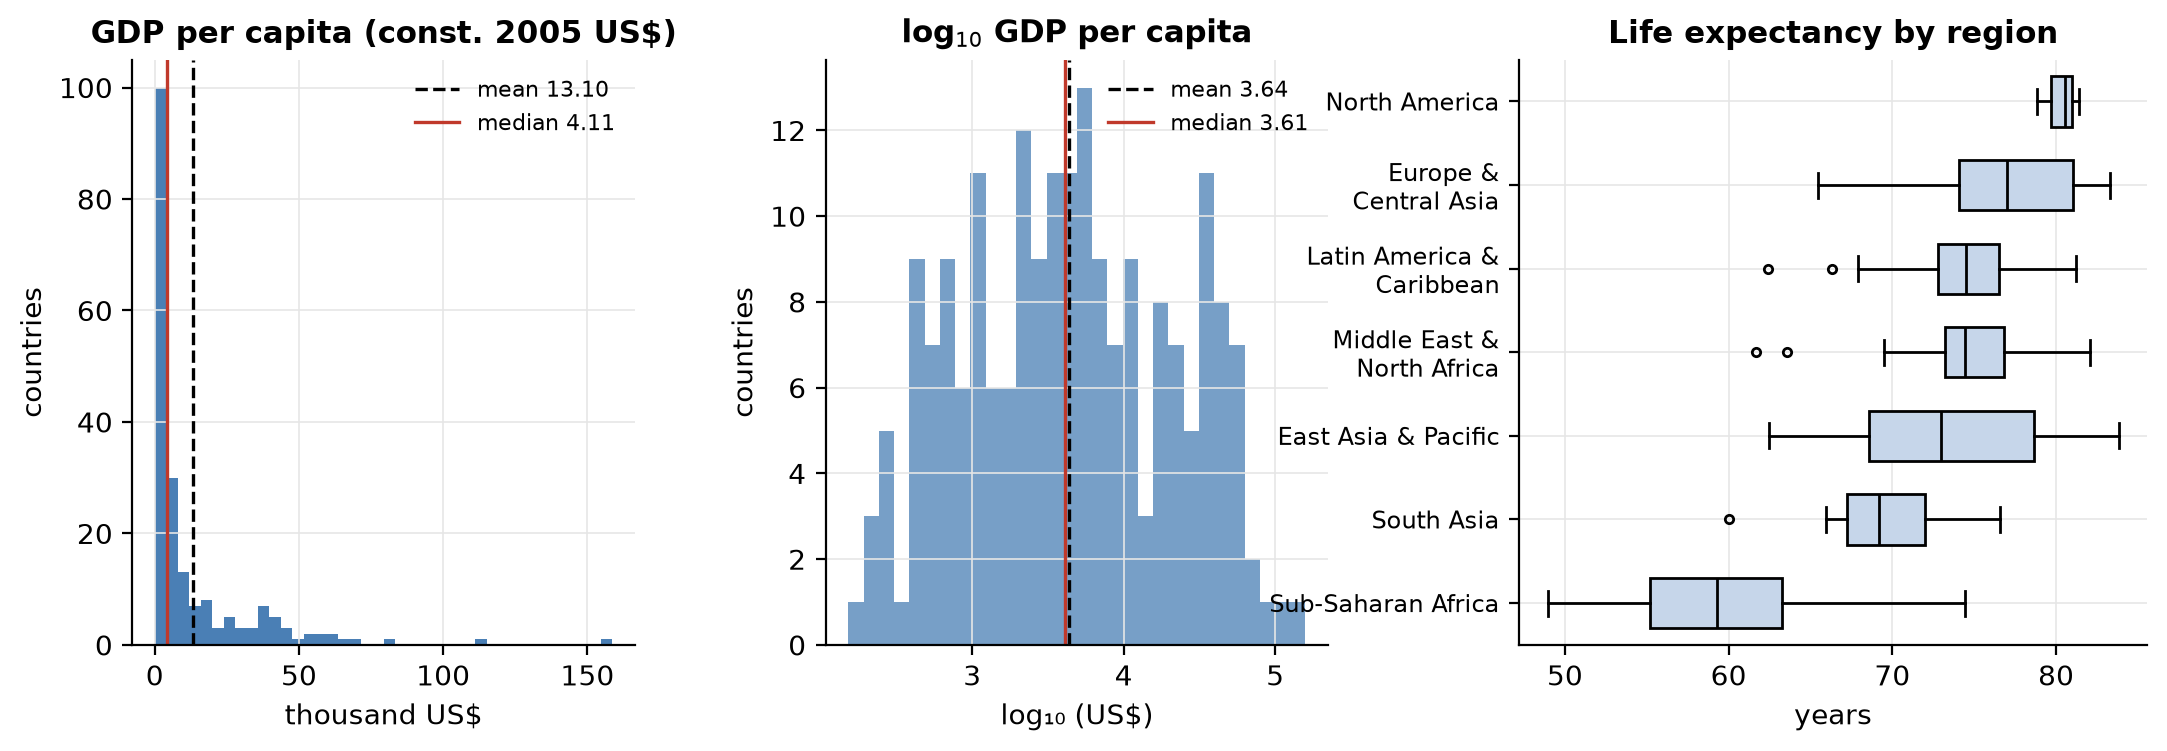
\includegraphics[width=\textwidth]{distributions.png}
\caption{Distributions of selected attributes in the snapshot. Skewed attributes such as income and CO$_2$ become approximately symmetric on a logarithmic scale.}\label{fig:dist}
\end{figure}

\paragraph{Missing values and their impact on the summary statistics.}
Missing values are the principal data-quality issue: 44.9\,\% of the cells of the country-year panel are empty. Most of this missingness is structural. Several series begin only around 1990 (internet, electricity, renewables), and others are derived from irregular household surveys (poverty, Gini index, literacy). Figure~\ref{fig:coverage} shows coverage by indicator and decade.

\begin{figure}[htbp]\centering
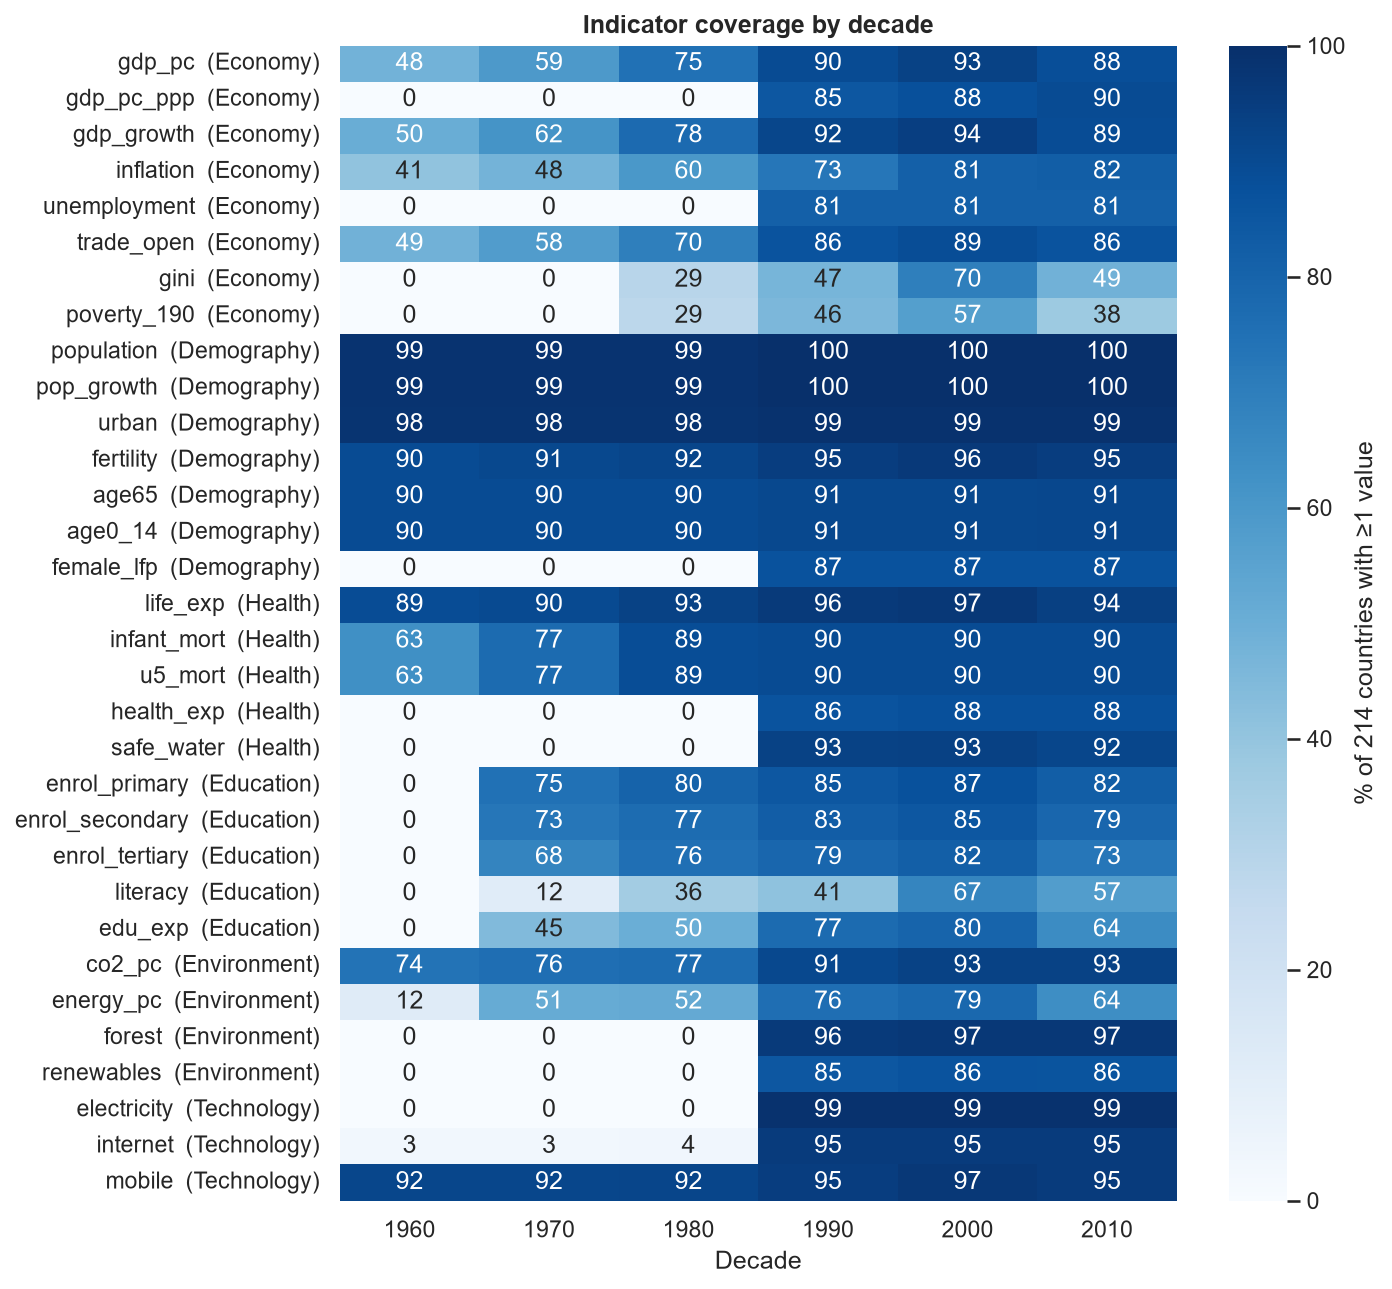
\includegraphics[width=0.85\textwidth]{01_coverage_heatmap.png}
\caption{Share of countries reporting each indicator by decade. Survey-based indicators (bottom rows) are sparse in every decade.}\label{fig:coverage}
\end{figure}

Missingness is not random \cite{little}; it depends on the income group (Figure~\ref{fig:missinc}). Poverty at \$1.90 per day is reported by 74--86\,\% of low- and lower-middle-income countries but by only 19\,\% of high-income countries, for which the World Bank does not measure extreme poverty. Literacy is reported by 44\,\% of high-income countries and child mortality by 75\,\%. Because missingness is related to income, which is itself an analysed variable, the mechanism is at least MAR and plausibly MNAR for survey indicators.

\begin{figure}[htbp]\centering
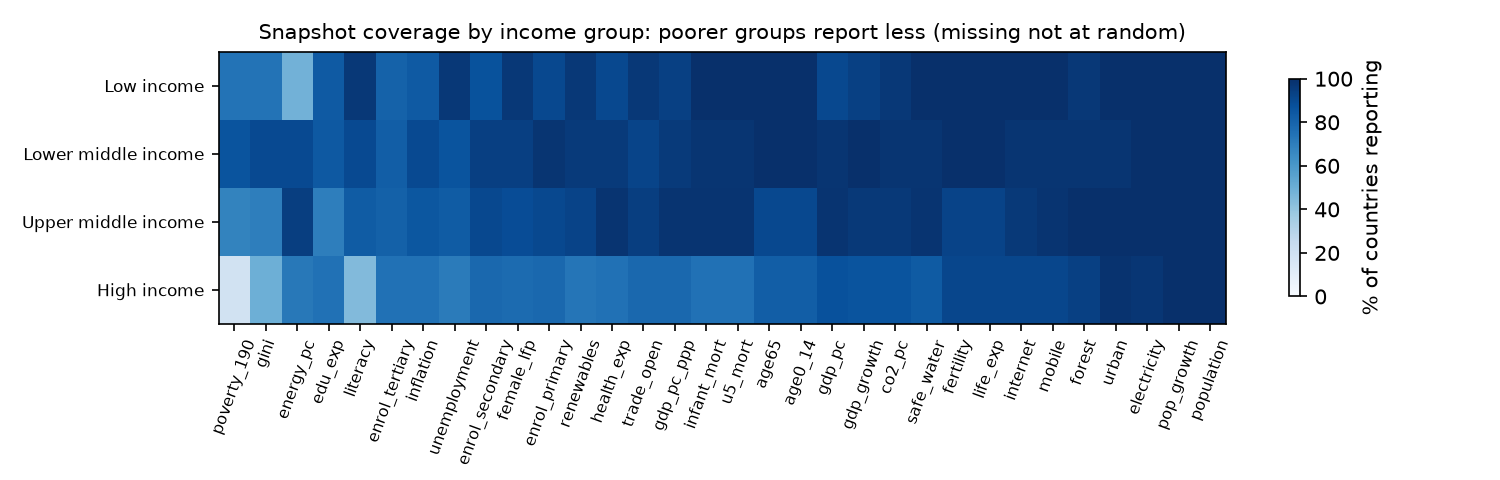
\includegraphics[width=\textwidth]{A2_missing_by_income.png}
\caption{Snapshot coverage by World Bank income group (darker cells indicate that more countries report). Coverage depends on income, so the reporting sample is biased.}\label{fig:missinc}
\end{figure}

To quantify the impact of missingness on the summary statistics, Table~\ref{tab:missing} compares the mean and median computed on reporting countries only with the same statistics after each missing value has been replaced by the median of the country's income group.

\begin{table}[htbp]\centering
\caption[Impact of missing values on summary statistics]{Impact of missing values on summary statistics. ``rep.'' denotes reporting countries only; ``imp.'' denotes values after income-group median imputation; Cov.\ is the percentage of countries reporting in each income group (LI, LMI, UMI, HI).}\label{tab:missing}
\tab{missing}
\end{table}

\begin{itemize}
\item For well-covered indicators (GDP, life expectancy, internet, CO$_2$; less than 8\,\% missing) the mean changes by less than 3\,\%, so missing values have a negligible effect.
\item For poverty, the reporting-only mean (19.2\,\%) overstates world poverty because high-income countries are absent. After imputation the mean falls by 30\,\% to 13.4\,\% and the median from 7.8\,\% to 1.8\,\%.
\item For literacy the bias has the opposite sign: high-income countries are under-represented, so the reporting-only mean (82.0\,\%) is too low (85.5\,\% after imputation). The mean of under-5 mortality is overstated by 8\,\% for the same reason.
\item Consequently, summary statistics of sparse, survey-based indicators describe the reporting countries rather than the world. Indicators with less than 60\,\% coverage are excluded from the exploratory analysis; the model suite applies a less restrictive 50\,\% threshold and retains poverty as a feature. The bias is stated wherever such indicators are used.
\end{itemize}

\begin{summary}[Key observations: summary statistics]
\begin{itemize}
\item Income, population, CO$_2$, energy use and mortality are strongly right-skewed (mean considerably above median), which motivates medians and logarithmic scales; percentages are bounded and left-skewed.
\item 44.9\,\% of panel cells are missing, mostly for structural reasons, and missingness depends on the income group.
\item The impact on summary statistics is negligible for well-covered indicators ($<3$\,\% change in the mean) but substantial for survey indicators: the poverty mean decreases by 30\,\% and the literacy mean increases by 4\,\% once non-reporting countries are taken into account.
\end{itemize}
\end{summary}

\subsection{Exploration of outliers, groups and notable values}

\paragraph{Outliers.} Values more than 1.5 interquartile ranges beyond the quartiles were flagged, using a logarithmic scale for skewed indicators (Table~\ref{tab:outliers}). In the raw panel, 29 country-years of \emph{hyperinflation} above 500\,\% were also identified (for example DR Congo 1994: 23,773\,\%; Bolivia 1985: 11,750\,\%; Peru 1990: 7,482\,\%).

\begin{table}[htbp]\centering
\caption{IQR outliers in the snapshot (indicators with at least one outlier).}\label{tab:outliers}
\tab{outliers}
\end{table}

Most outliers are genuine observations rather than errors. Small trading hubs (Hong Kong, Luxembourg, Singapore) record trade above 300\,\% of GDP; Gulf states have very high CO$_2$ emissions per capita; Libya's GDP fell by 24\,\% in a year of armed conflict; and several small island states spend heavily on health. Gross primary enrolment above 160\,\% (Gabon, Curaçao) reflects over-age pupils. Since the outliers are genuine, they are retained, robust statistics are used (medians, Spearman correlation, logarithmic scales) and hyperinflation years are flagged rather than removed (Section~\ref{sec:B}).

\paragraph{Groups of similar instances.} Countries form clear groups even before any model is fitted. The correlation matrix (Figure~\ref{fig:corr}) exhibits one large block: income, life expectancy, internet use, CO$_2$, energy use, water access and schooling correlate with GDP per capita at $|\rho| = 0.76$--$0.90$ and with each other. A principal component analysis of 15 standardised indicators assigns 63.5\,\% of the variance to the first component (Figure~\ref{fig:pca}), so that countries are arranged along a single dominant ``development axis''. Along this axis Sub-Saharan Africa forms a distinct low group, whereas oil exporters form a group with high income but comparatively poor health outcomes.

\begin{figure}[htbp]\centering
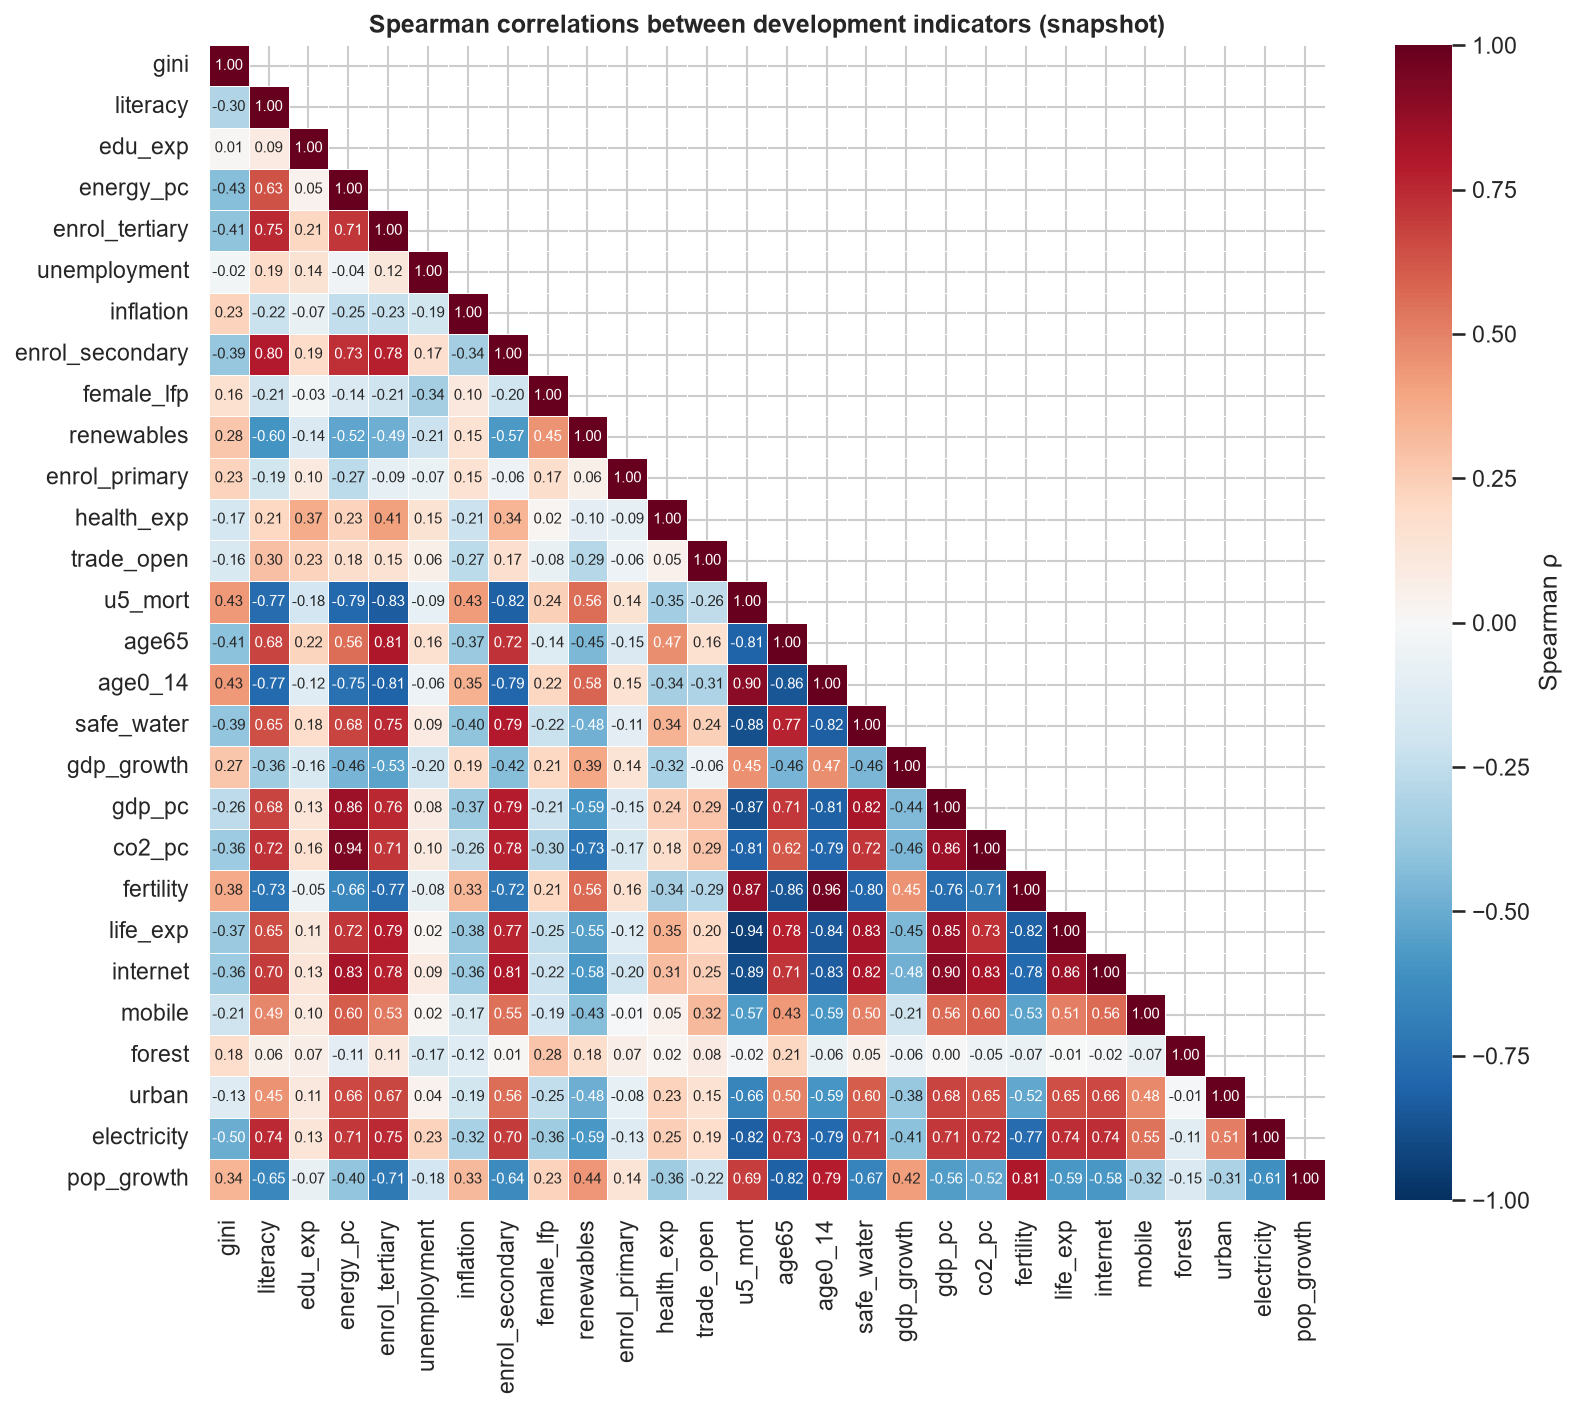
\includegraphics[width=0.82\textwidth]{16_correlation.png}
\caption{Spearman correlations between the indicators (snapshot). Development indicators form one strongly correlated block.}\label{fig:corr}
\end{figure}
\begin{figure}[htbp]\centering
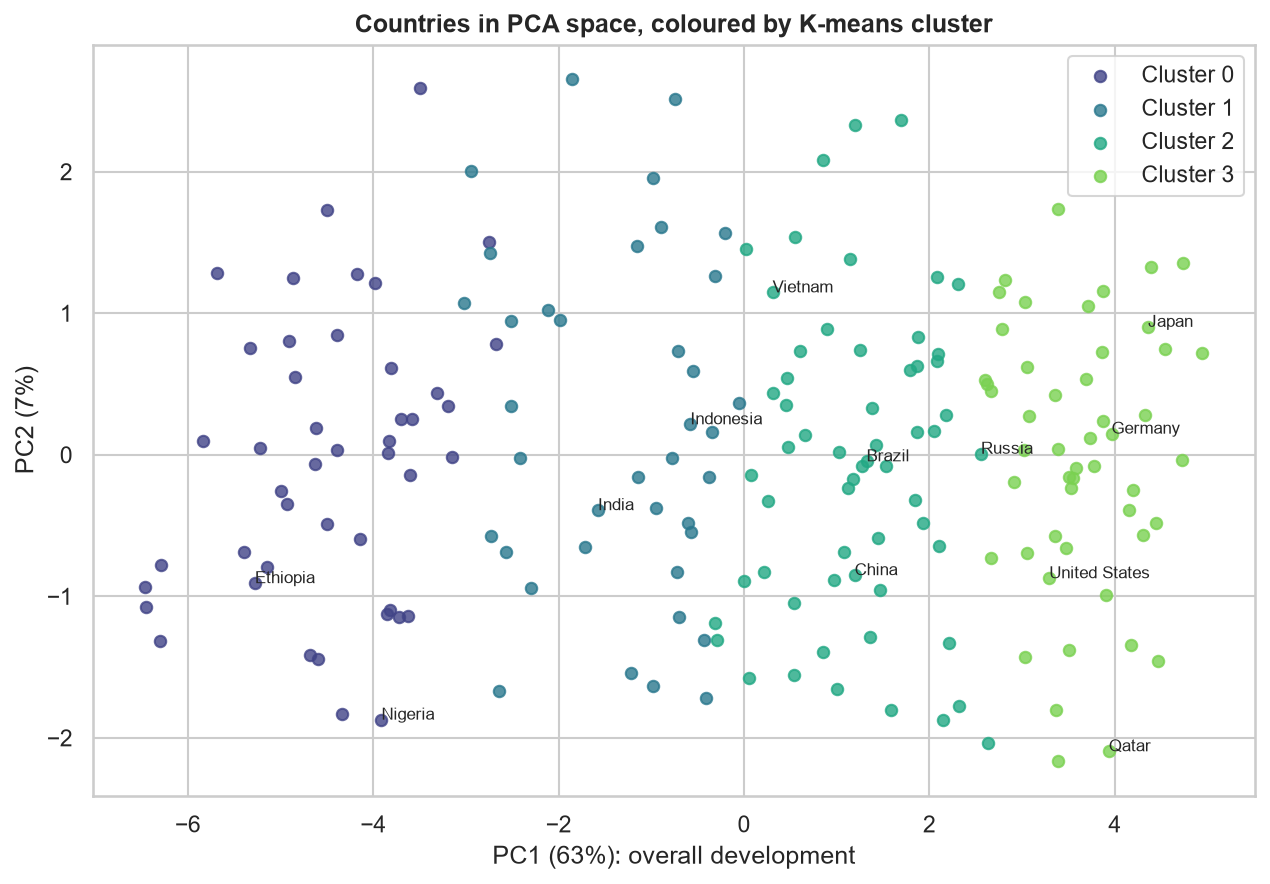
\includegraphics[width=0.68\textwidth]{21_pca_clusters.png}
\caption{PCA projection of 15 standardised indicators with K-means clusters. Countries are arranged along one principal axis.}\label{fig:pca}
\end{figure}

\paragraph{Notable attributes and values.}
\begin{itemize}
\item \emph{Life expectancy} is the most informative outcome. It increased in every region, by up to 30 years in South Asia (39 to 69 years), and the gap between high- and low-income countries narrowed from 30.1 to 20.8 years.
\item \emph{Fertility} distinguishes Sub-Saharan Africa from all other regions: it declined by only 28\,\% there (6.7 to 4.8 births per woman) compared with 60--67\,\% elsewhere. Niger (7.6) is the only fertility outlier.
\item \emph{GDP per capita} spans three orders of magnitude (US\$153 to US\$158,603), with a ratio of approximately 80 between the 90th and 10th percentiles.
\item \emph{Vietnam} is a notable value in almost every bivariate relationship. With a GDP per capita of US\$1,078 it records a life expectancy of 75.8 years, equal to that of China and Thailand, which are 3.5 times richer (Figure~\ref{fig:preston}).
\item Large negative deviations from the Preston curve are observed for Swaziland, Equatorial Guinea, Angola and South Africa, whose life expectancy is 15--20 years below the level predicted by income in the full-sample fit, reflecting the HIV epidemic and oil-based income. In the cross-validated income-only model of experiment E2.2, Somalia ranks fourth and South Africa fifth.
\end{itemize}

\begin{figure}[htbp]\centering
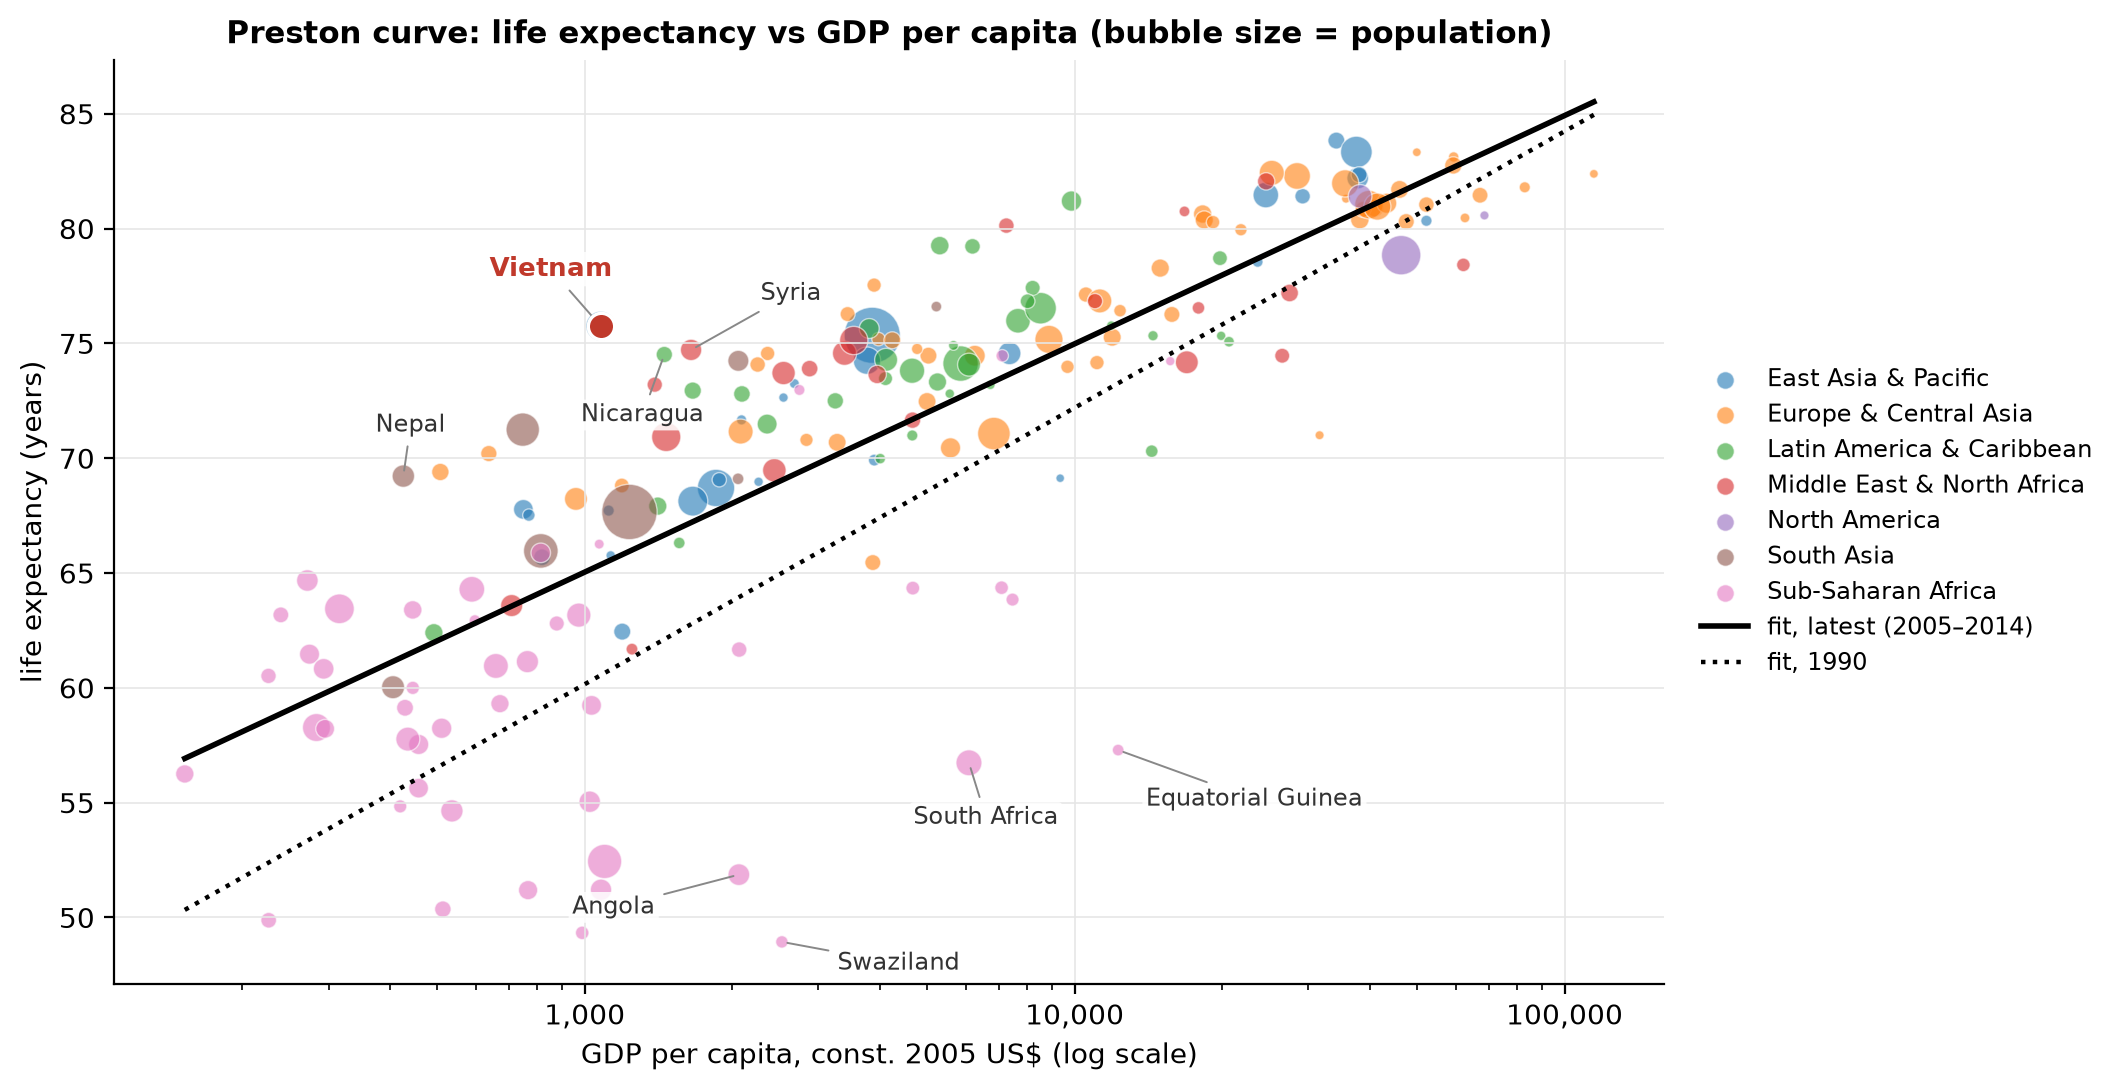
\includegraphics[width=1.00\textwidth]{preston_curve.png}
\caption{The Preston curve \cite{preston}: life expectancy against log GDP per capita. Vietnam (red) lies furthest above the fitted curve.}\label{fig:preston}
\end{figure}

\paragraph{Impact of missing values on the exploration.} Table~\ref{tab:corr} recomputes key correlations under pairwise deletion and after imputation.

\begin{table}[htbp]\centering
\caption{Spearman $\rho$ under pairwise deletion and under income-group median imputation.}\label{tab:corr}
\tab{corr}
\end{table}

\begin{itemize}
\item For well-covered pairs the correlation changes by at most 0.03, so the exploratory findings are robust to missingness.
\item For sparse indicators imputation alters the conclusion: the correlation between the Gini index and income changes from $-0.26$ to $-0.42$. Because income-group medians are themselves a function of income, imputation artificially strengthens relationships with income. Imputed values are therefore never used for correlation or regression involving sparse indicators.
\item Listwise deletion is not a viable alternative. Only 69 of the 214 countries report all 32 indicators, and 147 report all 15 clustering indicators. Removing incomplete countries would disproportionately exclude poor and small countries and bias every result towards high-income countries. This observation motivates the missing-value strategy described in Section~\ref{sec:B}.
\end{itemize}

\begin{summary}[Key observations: exploration]
\begin{itemize}
\item Outliers are predominantly genuine (trade hubs, Gulf CO$_2$ emissions, conflicts, hyperinflation); they are retained and analysed with robust methods, and 29 hyperinflation years are flagged.
\item The indicators form one correlated block around income, and countries lie along one principal axis (PC1 = 63.5\,\%), with Sub-Saharan Africa and oil exporters as distinct groups.
\item Life expectancy (strong convergence), fertility (the Sub-Saharan exception), GDP (very large dispersion) and Vietnam (the largest positive deviation from the Preston curve) are the most notable attributes and values.
\item Missing values have little effect on well-covered correlations, but imputation biases sparse ones (Gini: $-0.26$ to $-0.42$), and listwise deletion would retain only 69 countries.
\end{itemize}
\end{summary}

% ================================================================== 4
\section{Data preprocessing}\label{sec:B}
Each preprocessing technique was selected to address a specific problem identified in Section~\ref{sec:A}. All four classical groups of techniques \cite{han} were applied, complemented by two procedures specific to the modelling task. Table~\ref{tab:findings} maps the problems to the techniques, and Table~\ref{tab:prep} summarises the effect of each step.

\begin{table}[htbp]\centering\small
\caption{Problems identified during exploration and the preprocessing techniques chosen to address them.}\label{tab:findings}
\begin{adjustbox}{max width=\textwidth}\begin{tabular}{p{6.3cm}lp{6.3cm}}
\toprule
Problem (Section~\ref{sec:A}) & Group & Technique \\
\midrule
1,344 sparse indicators, 5.66\,M rows, 574\,MB & Reduction & attribute selection (32 indicators), chunked filtering \\
33 aggregates mixed with countries & Cleaning & removal of aggregates (empty \var{Region}) \\
metadata stored in separate files & Integration & joins on \var{CountryCode} and \var{IndicatorCode} \\
long format with one row per value & Transformation & reshaping to a wide panel and snapshot \\
44.9\,\% of cells missing, not at random & Cleaning & short-gap interpolation, 10-year snapshot, coverage threshold, method-specific imputation \\
strong right skew (skewness 1.2--8.9) & Transformation & $\log_{10}$ transform \\
scales differing by orders of magnitude & Transformation & z-score standardisation \\
genuine extremes and hyperinflation & Cleaning & retain, flag hyperinflation, robust statistics \\
one correlated block of indicators & Reduction & PCA \\
near-definitional feature pairs & Leakage control & removal of leaking features per target \\
\bottomrule
\end{tabular}\end{adjustbox}
\end{table}

\begin{table}[htbp]\centering\small
\caption{Effect of the preprocessing pipeline.}\label{tab:prep}
\begin{adjustbox}{max width=\textwidth}\begin{tabular}{lll}
\toprule
Step & Technique & Result \\
\midrule
Reduction & chunked reading, filtering of 32 of 1,344 indicators & 5.66\,M $\to$ 247,446 rows, 34.9\,MB in memory \\
Cleaning & separation of aggregates & 210,443 country rows; 37,003 aggregate rows set aside \\
Cleaning & duplicates / non-finite / out-of-domain values & 0 / 0 / 0 found \\
Cleaning & flagging of hyperinflation ($>$\,500\,\%) & 29 country-years flagged and retained \\
Integration & joins with \texttt{Country.csv} and \texttt{Series.csv} & region, income group, names and topics attached \\
Transformation & long $\to$ wide & panel of 11,935 country-years $\times$ 32 \\
Cleaning & interpolation of gaps $\le$\,3 years & missing cells 44.9\,\% $\to$ 42.1\,\% \\
Reduction & 2005--2014 snapshot & 214 countries $\times$ 32, median data year 2014 \\
Reduction & coverage threshold & exploration: 60\,\%, 31 indicators (poverty excluded); model suite: 50\,\% \\
Transformation & $\log_{10}$, standardisation & approximately symmetric, comparable features \\
Reduction & PCA (15 indicators) & PC1 63.5\,\%, PC1 + PC2 70.8\,\% \\
\bottomrule
\end{tabular}\end{adjustbox}
\end{table}

\subsection{Data cleaning}
\begin{itemize}
\item \emph{Removal of aggregates.} The 33 aggregates would double-count countries; they are identified by an empty \var{Region} and set aside.
\item \emph{Validation.} No duplicate (country, indicator, year) keys, no infinite values and no values outside the valid domain (for example percentages outside 0--100 where applicable) were found.
\item \emph{Outliers.} Genuine extremes are retained (Section~\ref{sec:A}). The 29 hyperinflation years are flagged rather than deleted, and inflation is log-transformed for modelling.
\item \emph{Missing values} are treated according to their type:
  \begin{enumerate}
  \item only short internal gaps ($\le$\,3 years) are linearly interpolated, and no value is extrapolated (44.9\,\% $\to$ 42.1\,\% missing);
  \item for the cross-country snapshot, the latest value within a ten-year window (2005--2014) is used;
  \item values are imputed only where a method requires complete input. The model suite uses the median of the training fold, fitted inside each cross-validation fold so that no information from test countries leaks into training; clustering and the missing-data analysis use income-group medians computed on the full sample;
  \item indicators below 60\,\% coverage are excluded from the exploratory analysis (poverty at \$1.90, 55\,\%), whereas the model suite applies a 50\,\% threshold and retains poverty as a feature;
  \item group trends are reported only for years in which at least 30\,\% of the group's countries report.
  \end{enumerate}
\end{itemize}
As a result, no country is discarded because of isolated gaps: the model suite uses 185--204 countries per target and the clustering 192 countries, compared with 69 under listwise deletion. Experiment E1.3 (Section~\ref{sec:conv}) verifies that the conclusions do not depend on the changing set of reporting countries.

\subsection{Data integration}
The three files are joined on their keys. \texttt{Indicators.CountryCode} $\to$ \texttt{Country.CountryCode} adds \var{ShortName}, \var{Region} and \var{IncomeGroup}, and \texttt{Indicators.IndicatorCode} $\to$ \texttt{Series.SeriesCode} adds the indicator name, topic and unit. The two high-income groups (OECD and non-OECD) are merged into a single ``High income'' level, which yields an ordinal income attribute with four levels. Each indicator receives a short alias (for example \var{SP.DYN.LE00.IN} $\to$ \var{life\_exp}) and is assigned to a theme.

\subsection{Data transformation}
\begin{itemize}
\item \emph{Reshaping.} The long table is converted into a wide country-year panel (one column per indicator) and a wide country snapshot.
\item \emph{Logarithmic transformation.} Right-skewed attributes are transformed with $\log_{10}$. The model suite transforms GDP per capita (market and PPP), CO$_2$, energy use, trade and inflation (signed, $\log_{10}(1+|x|)$); the clustering transforms GDP per capita, CO$_2$, energy use, trade and under-5 mortality. The transformation linearises relationships such as the Preston curve and reduces the leverage of extreme values.
\item \emph{Standardisation.} Features are converted to z-scores before PCA, clustering, distance computations and linear models; in the model suite the scaler is fitted inside each training fold.
\item \emph{Derived attributes.} Annual growth rates (CAGR and log growth) are derived for the convergence analysis, country and year means for the fixed-effects model, and out-of-fold residuals as a measure of performance relative to income.
\end{itemize}

\subsection{Data reduction}
\begin{itemize}
\item \emph{Attribute selection.} The 1,344 indicators are reduced to 32 on the basis of domain knowledge and coverage, then to 31 by the 60\,\% coverage threshold of the exploratory analysis. Fifteen indicators are used for clustering and ten social indicators, excluding income, for the similarity analysis (E3.2).
\item \emph{Instance reduction.} Chunked filtering reduces 5.66\,M rows to 247k without loading the 574\,MB file into memory at once; the snapshot reduces 55 years to one value per country.
\item \emph{Dimensionality reduction.} PCA on 15 standardised indicators yields a first component that explains 63.5\,\% of the variance and a second that explains 7.3\,\%. PC1 loads almost equally on income, health, schooling, internet use and CO$_2$, which confirms a single dominant development dimension; PC2 is driven mainly by forest cover.
\end{itemize}

\subsection{Leakage control and validation design}
\begin{itemize}
\item \emph{Removal of near-definitional features.} For each target, features that are near-definitional of it are removed: infant and under-5 mortality when predicting life expectancy; age structure and population growth when predicting fertility; PPP GDP and GDP growth when predicting GDP; primary and tertiary enrolment when predicting secondary enrolment; energy use when predicting CO$_2$; and mobile subscriptions when predicting internet use.
\item \emph{Country-grouped cross-validation.} Folds are formed by country, so that no country appears in both the training and the test data; in the panel, its other years would otherwise leak information.
\item \emph{Balanced panel and population weights} (E1.3) are used as robustness checks against changing coverage.
\end{itemize}

% ================================================================== 5
\section{Methodology}\label{sec:method}

\subsection{Analytical framework}
Table~\ref{tab:actions} lists the data-mining tasks and links each to a research question. Tasks 1, 3 and 4 originate from the exploratory notebook and the model suite; tasks 2 and 5--8 consist of, or combine notebook results with, nine experiments (E1.1--E3.3) implemented in the \texttt{wdi/story/} package.

\begin{table}[htbp]\centering\small
\caption{Data-mining tasks and the research questions they address.}\label{tab:actions}
\begin{tabular}{p{0.4cm}p{3.3cm}p{4.9cm}p{4.6cm}p{0.8cm}}
\toprule
\# & Task & Method & Question & RQ \\
\midrule
1 & Trend analysis & group medians by income group and region & How did each theme change since 1960? & 1 \\
2 & Inequality and convergence & Gini, p90/p10 ratio, $\sigma$- and $\beta$-convergence (E1.1--E1.3) & Are countries becoming more alike? & 1 \\
3 & Association & Spearman correlation, Preston and Kuznets curves & Which indicators move with income? & 2 \\
4 & Prediction (regression) & 19 regressors $\times$ 6 targets, country-grouped 5-fold CV, 3--5 seeds & How predictable is each theme? & 2 \\
5 & Residual and panel analysis & income-only models (E2.1, E2.2), two-way fixed effects (E2.3) & How much does income explain, and which countries deviate? & 2 \\
6 & Clustering & K-means, Gaussian mixture, Ward; PCA (E3.1) & Do data-driven groups match income groups? & 3 \\
7 & Similarity search & nearest neighbours in social-indicator space (E3.2) & Which countries is Vietnam most similar to? & 3 \\
8 & Gap analysis & standardised distance to cluster medians (E3.3) & What separates Vietnam from the next group? & 3 \\
\bottomrule
\end{tabular}
\end{table}

\subsection{Convergence measures (RQ1)}
$\sigma$-convergence (E1.1) is measured by the cross-country coefficient of variation of indicator $x$ in year $t$,
\begin{equation}
\mathrm{CV}_t = \frac{s_t}{\bar{x}_t},
\end{equation}
where $s_t$ and $\bar{x}_t$ are the standard deviation and mean across countries. Only years in which more than 100 countries report are used. $\beta$-convergence (E1.2) is estimated by the cross-sectional regression
\begin{equation}
g_i = \alpha + \beta\, x_{i,1990} + \varepsilon_i,
\end{equation}
where $g_i$ is the annual change of country $i$ between 1990 and the last year with more than 100 reporting countries. For GDP, $g_i$ is the log growth rate in percent per year and $x_{i,1990}$ the $\log_{10}$ level; for the other indicators, $g_i$ is the change in units per year. A negative $\beta$ indicates catch-up; 95\,\% confidence intervals are based on the $t$ distribution. Experiment E1.3 recomputes the change in CV between 1990 and 2013 on (a) all reporting countries, (b) a balanced panel of countries reporting in both years and (c) the balanced panel weighted by population. A change of more than 5\,\% is classified as convergence or divergence.

\subsection{Predictive modelling and residuals (RQ2)}
For each theme one target indicator is predicted from the remaining non-leaking indicators. Nineteen regressors are compared, ranging from linear models (OLS, Ridge, Lasso, ElasticNet, Huber, Bayesian Ridge) through kernel and neighbourhood methods (SVR, KNN), a neural network (MLP) and tree models (decision tree, random forest \cite{breiman}, extra trees, gradient boosting, histogram gradient boosting, AdaBoost, XGBoost \cite{xgb}, LightGBM \cite{lgbm}) to two ensembles (voting and stacking). Experiment E2.1 decomposes the explained variance into three layers: (i) Ridge regression on log GDP per capita only, (ii) Ridge regression on all non-leaking features and (iii) the best model of the suite.

The residual of country $i$ (E2.2) is computed from the income-only model as
\begin{equation}
e_i = y_i - \hat{y}_i^{(-k(i))},
\end{equation}
where $\hat{y}_i^{(-k(i))}$ is the prediction of a model fitted on the folds that do not contain country $i$. For log-transformed targets the residual is reported as the ratio of actual to predicted values.

To separate the between-country from the within-country association (E2.3), a two-way fixed-effects model \cite{wooldridge} is estimated on the 1990--2014 panel:
\begin{equation}
\mathrm{LE}_{it} = \beta \log_{10}\mathrm{GDPpc}_{it} + \alpha_i + \gamma_t + \varepsilon_{it},
\end{equation}
where $\alpha_i$ and $\gamma_t$ are country and year effects. Standard errors are clustered by country. The fixed-effects slope is compared with a between-country regression on country means and with pooled OLS.

\subsection{Clustering, similarity and gap analysis (RQ3)}
K-means, Gaussian mixture models and Ward agglomerative clustering are applied to 15 standardised indicators for the 192 countries with at least 70\,\% coverage (2.5\,\% of cells imputed with income-group medians). Clusters are ordered and named by their median GDP per capita (low development, transition, emerging, advanced). Experiment E3.1 repeats each algorithm with 20 seeds. Experiment E3.2 retrieves the five nearest neighbours of Vietnam by Euclidean distance (i) on GDP per capita alone and (ii) on ten standardised social indicators that exclude income. Experiment E3.3 expresses the difference between Vietnam and the median of a cluster in units of the cross-country standard deviation,
\begin{equation}
\mathrm{gap}_j = \frac{x_{\mathrm{VN},j} - \operatorname{median}_{c}(x_j)}{s_j}.
\end{equation}

\subsection{Evaluation protocol}
\begin{itemize}
\item \emph{Regression metrics.} The coefficient of determination $R^2 = 1 - \sum_i(y_i-\hat y_i)^2 / \sum_i(y_i-\bar y)^2$, the mean absolute error (MAE) and the root mean squared error (RMSE) are computed on out-of-fold predictions only.
\item \emph{Validation scheme.} Five-fold \texttt{GroupKFold} by country, repeated with five seeds (snapshot) or three seeds (panel). Results are reported as mean $\pm$ standard deviation across seeds. Imputation and scaling are fitted inside each training fold.
\item \emph{Clustering metrics.} The silhouette coefficient $s(i) = (b_i - a_i)/\max(a_i, b_i)$ \cite{rousseeuw}, where $a_i$ is the mean intra-cluster distance and $b_i$ the mean distance to the nearest other cluster; the adjusted Rand index (ARI) \cite{hubert} for agreement between two partitions (1 for identical partitions, 0 for chance agreement); and the agreement with the World Bank income groups, defined as the share of countries that belong to the dominant income group of their cluster.
\item \emph{Statistical inference.} Slopes are reported with 95\,\% confidence intervals and $p$-values; panel standard errors are clustered by country.
\end{itemize}

\subsection{Reproducibility and use of generative AI tools}
All computations are implemented in Python (pandas \cite{pandas}, NumPy, SciPy, scikit-learn \cite{sklearn}, XGBoost, LightGBM); report figures are produced with Matplotlib and Seaborn, and the web application with Plotly and Streamlit \cite{streamlit}. Random seeds are fixed, all intermediate results are stored as CSV files in \texttt{results/}, and the tables of this report are generated directly from these files by \texttt{report/make\_tables.py}. Automated tests verify the headline numbers and the rendering of every page of the application (Section~\ref{sec:app}).

A generative AI assistant was used to support code refactoring, to edit the wording of this report and to cross-check reported figures against the result files. All analyses were specified and executed by the group, every number in this report is traceable to the result files listed in Appendix~\ref{app:repo}, and the group takes full responsibility for the content.

% ================================================================== 6
\section{Results}\label{sec:results}

\subsection{RQ1: Trends and convergence}\label{sec:conv}

\paragraph{Trends by theme.} Group-median trends (Figure~\ref{fig:trends}) indicate broad social progress. Life expectancy increased in every region, primary enrolment became nearly universal, and mobile subscriptions reached about 64 per 100 people even in low-income countries. Over 1990--2014, median GDP per capita grew by 2.1\,\% per year in upper-middle-income and 1.7\,\% per year in lower-middle-income countries, compared with 0.6\,\% per year in high-income countries.

\begin{figure}[htbp]\centering
\begin{subfigure}{\textwidth}\centering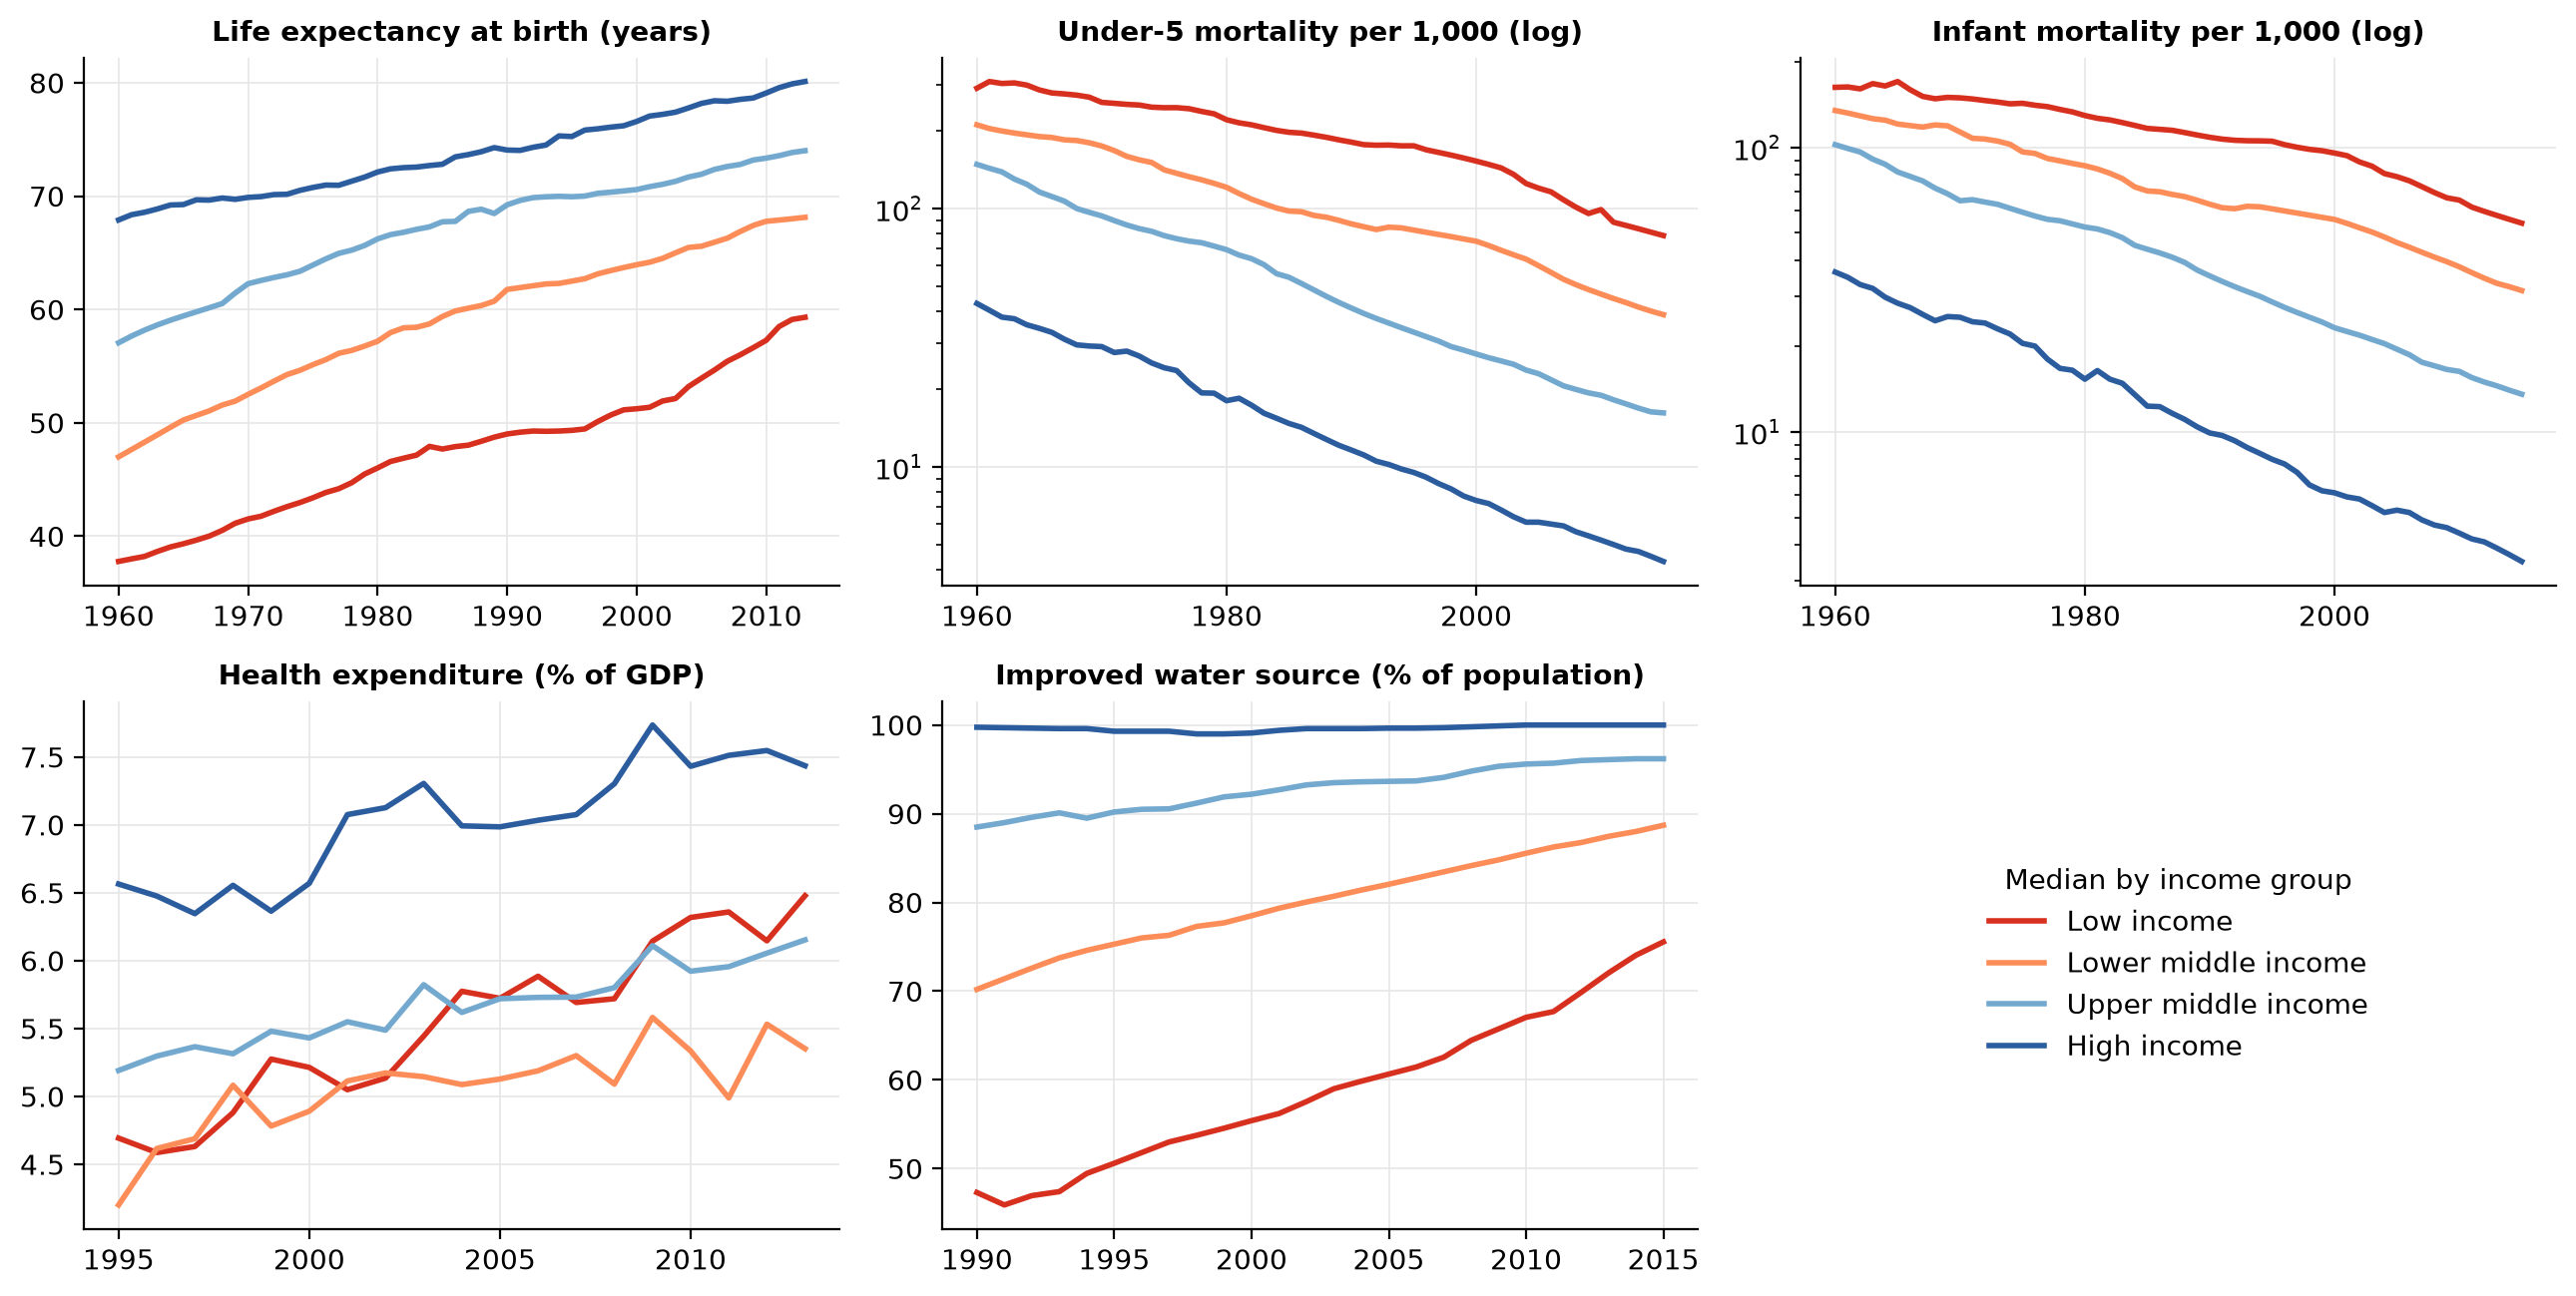
\includegraphics[width=0.92\textwidth]{trend_health.png}\caption{Health, median by income group}\end{subfigure}\\[4pt]
\begin{subfigure}{\textwidth}\centering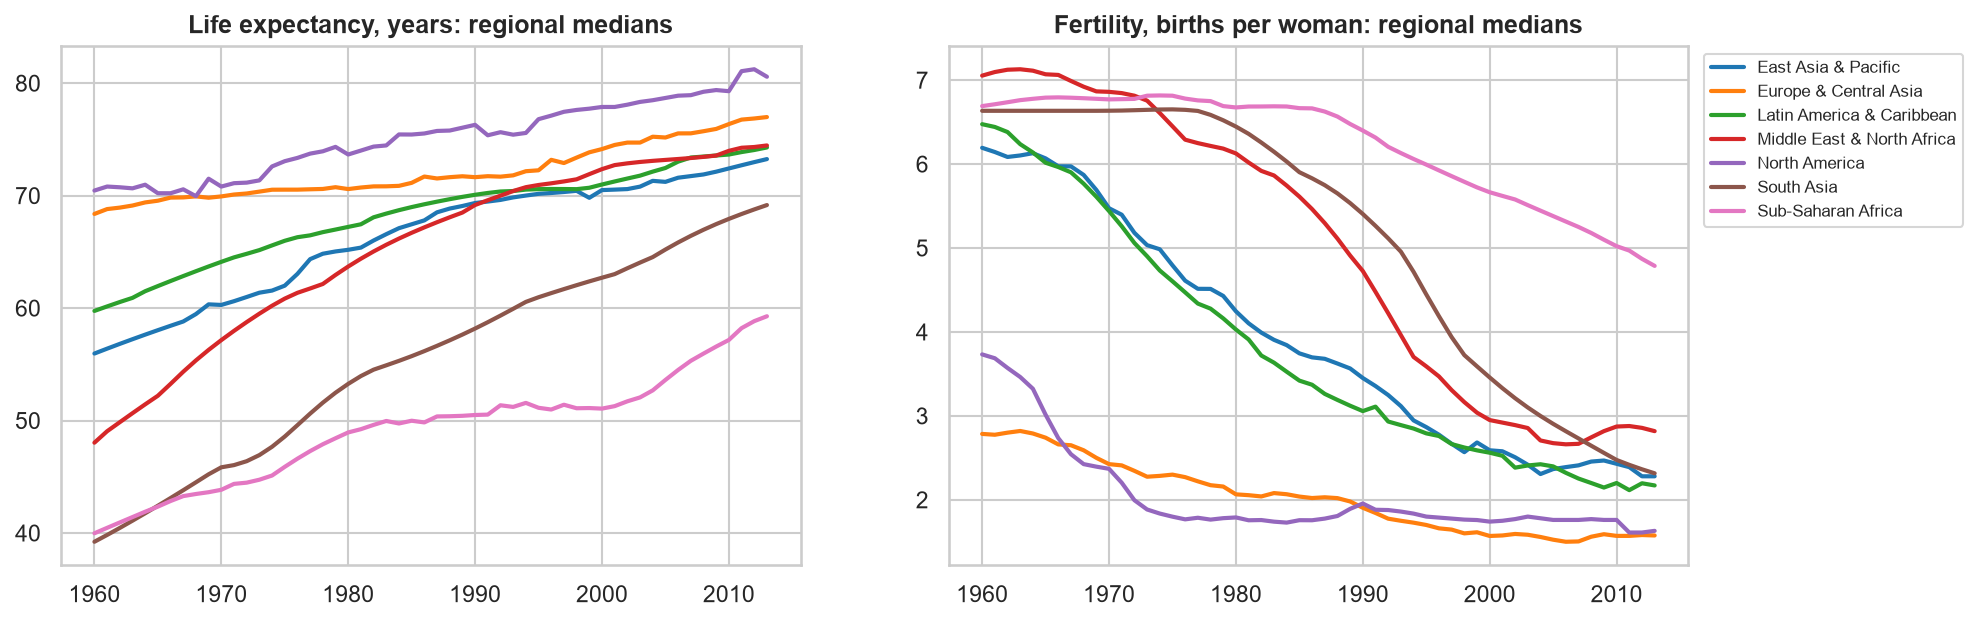
\includegraphics[width=0.92\textwidth]{10_trend_regions.png}\caption{Regions: life expectancy and fertility}\end{subfigure}
\caption{Group-median trends. All regions gained life expectancy, whereas the decline in fertility stalled only in Sub-Saharan Africa.}\label{fig:trends}
\end{figure}

\paragraph{$\sigma$-convergence (E1.1).} Social indicators converged markedly, whereas the dispersion of income remained almost unchanged (Figure~\ref{fig:sigma}, Table~\ref{tab:sigma}). The cross-country CV fell by 47\,\% for life expectancy, 67\,\% for primary enrolment and 85\,\% for internet use, while the CV of GDP per capita was 1.46 at both ends of the period.

\begin{figure}[htbp]\centering
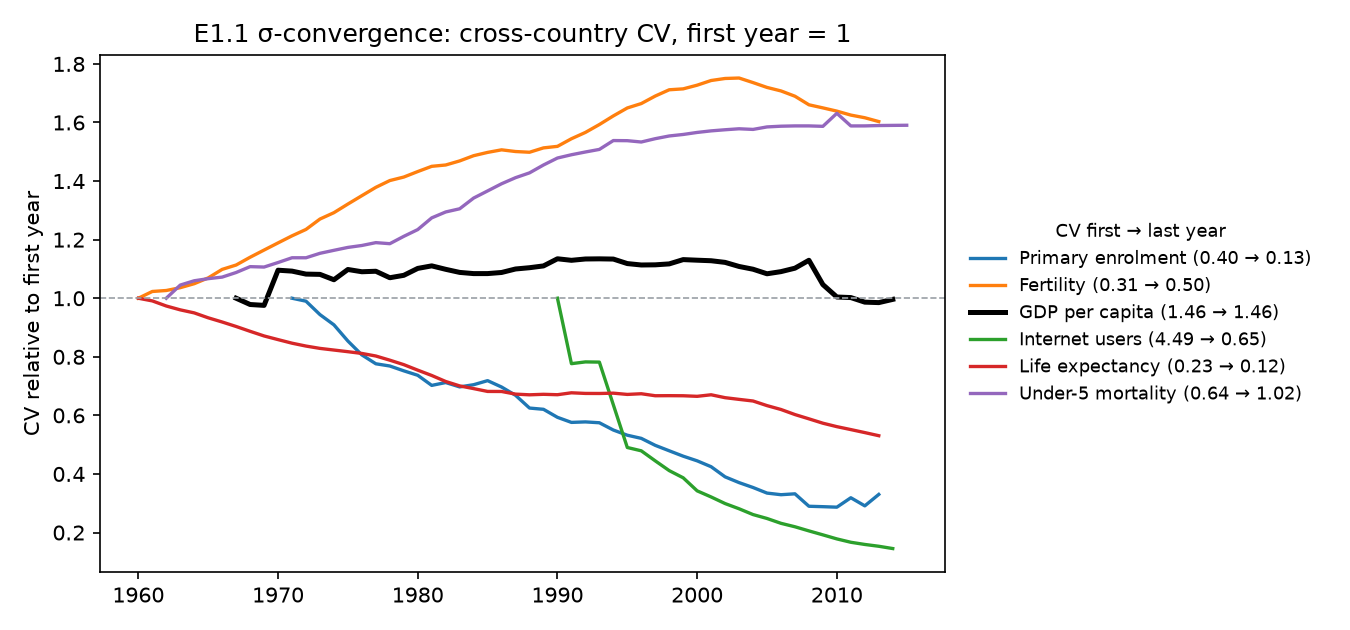
\includegraphics[width=0.85\textwidth]{E1_1_sigma.png}
\caption{E1.1: cross-country CV relative to the first year. Health, schooling and internet use converge; GDP remains flat; fertility diverges.}\label{fig:sigma}
\end{figure}

\begin{table}[htbp]\centering
\caption{E1.1: $\sigma$-convergence (years with more than 100 reporting countries).}\label{tab:sigma}
\tab{sigma}
\end{table}

Two qualifications apply. First, the apparent divergence of under-5 mortality is relative: as high-income countries approach zero, the ratio between countries increases even though absolute gaps decrease. Second, the flat GDP line compares 101 countries in 1967 with 179 in 2014; on a constant set of countries over 1990--2013 the CV decreases by 5\,\% (E1.3).

\paragraph{$\beta$-convergence (E1.2).} Countries with lower initial levels of health, schooling and fertility improved faster (Figure~\ref{fig:beta}, Table~\ref{tab:beta}): $\beta$ is negative and significant ($r = -0.52$ to $-0.85$, $p < 0.001$). For GDP per capita the relationship is weak and not significant at the 5\,\% level ($r = -0.15$, $p = 0.054$). Catch-up in income was driven by a limited number of countries, notably China (9.2\,\% per year), Vietnam (5.3--5.5\,\%), Lao PDR and India.

\begin{figure}[htbp]\centering
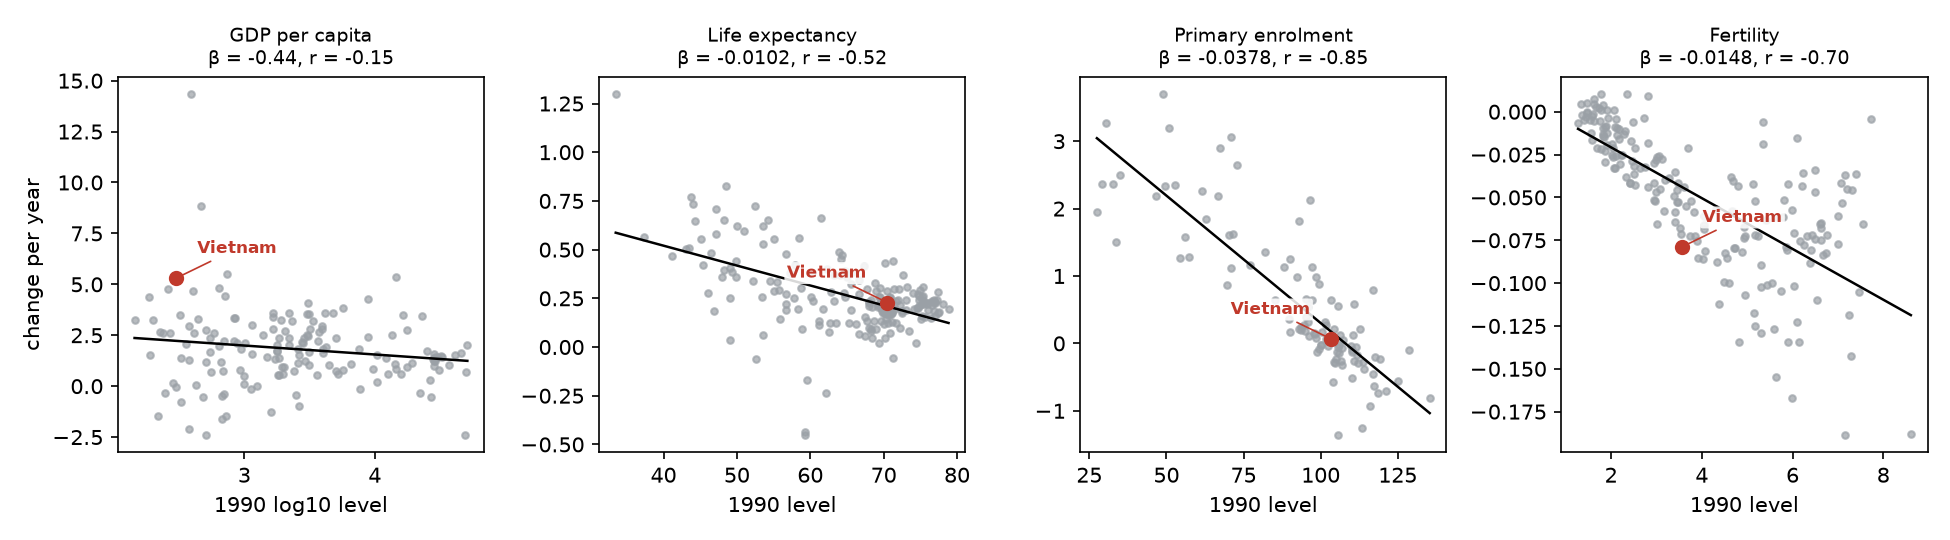
\includegraphics[width=\textwidth]{E1_2_beta.png}
\caption{E1.2: annual change against the 1990 level. Vietnam (red) grew considerably faster than its 1990 income level would predict.}\label{fig:beta}
\end{figure}
\begin{table}[htbp]\centering
\caption{E1.2: $\beta$-convergence.}\label{tab:beta}
\tab{beta}
\end{table}

\paragraph{Robustness to coverage (E1.3).} Because poorer countries report less often, convergence could be an artefact of countries entering the dataset. Table~\ref{tab:robust} shows that the direction of change holds on a balanced panel and with population weights. One correction is necessary: more than half of the small decline in the CV of GDP since 1990 is a composition effect ($-13$\,\% with all reporting countries, $-5$\,\% on the balanced panel), and the population-weighted decline largely reflects growth in China and India.

\begin{table}[htbp]\centering
\caption{E1.3: change in CV between 1990 and 2013 on three samples.}\label{tab:robust}
\tab{robust}
\end{table}

\begin{summary}[Answer to RQ1]
Development indicators improved almost everywhere, and countries became considerably more similar in health and schooling (H1 supported). Income did not converge: the dispersion of GDP per capita was essentially unchanged and $\beta$-convergence was not significant (H2 supported). Sub-Saharan Africa is the main exception to the demographic transition, with fertility declining by 28\,\% against 60--67\,\% elsewhere.
\end{summary}

\subsection{RQ2: The explanatory power of income}

\paragraph{Model suite.} Each theme has one target that is predicted from the other indicators after removal of leaking features. Table~\ref{tab:models} compares the linear baseline, random forest and the best of the 19 models.

\begin{table}[htbp]\centering
\caption[Model suite: cross-validated $R^2$, MAE and RMSE]{Model suite (bold: best $R^2$, and gains of at least 0.1 over the linear model). Linear and RF columns give the mean $R^2$ over seeds. The best model is the one with the highest mean $R^2$, reported as mean $\pm$ standard deviation over seeds (five for the snapshot, three for the panel); the $\pm$ term therefore measures seed-to-seed variation. Each seed's $R^2$ uses out-of-fold predictions pooled over the five country-grouped folds. MAE and RMSE are reported for the best model in target units ($\log_{10}$ for GDP and CO$_2$; years for life expectancy; births per woman for fertility; percentage points for enrolment and internet use).}\label{tab:models}
\tab{models}
\end{table}

\begin{itemize}
\item All six themes are predicted with high accuracy ($R^2$ 0.77--0.90); life expectancy is predicted with a mean absolute error of 2.7 years.
\item Ensemble methods (voting, stacking, extra trees) achieve the highest scores, but their advantage over a linear model is small: 0.03--0.09 in $R^2$ for every snapshot theme. The exception is internet use in the panel (0.69 to 0.90), where adoption follows an S-shaped time path that a linear model cannot represent.
\item The seed-to-seed standard deviation of the best models is small ($\le$\,0.009), so differences above approximately 0.02 can be regarded as meaningful.
\item In a simple life-expectancy model, log GDP alone yields $R^2 = 0.64$ (MAE 3.6 years); seven additional indicators raise this to 0.76 (MAE 2.9), and a random forest \cite{breiman} attains 0.76 (MAE 2.8). Since the relationship is essentially linear in log income, the interpretable model is preferred.
\end{itemize}

\begin{table}[htbp]\centering
\caption{Permutation importance (decrease in $R^2$ on 25\,\% of countries held out, best snapshot model).}\label{tab:imp}
\tab{importance}
\end{table}
The permutation importances (Table~\ref{tab:imp}) indicate that development indicators largely substitute for one another: income is best predicted by internet use and CO$_2$, life expectancy by fertility and electricity access, and CO$_2$ by income.

\paragraph{Share explained by income (E2.1).} Income alone yields cross-validated $R^2$ values of 0.51--0.77 (mean 0.63), approximately three quarters of the mean of 0.82 achieved by the best model (Figure~\ref{fig:r2}, Table~\ref{tab:r2}). The remaining indicators add 0.16 on average, and model complexity a further 0.03.

\begin{figure}[htbp]\centering
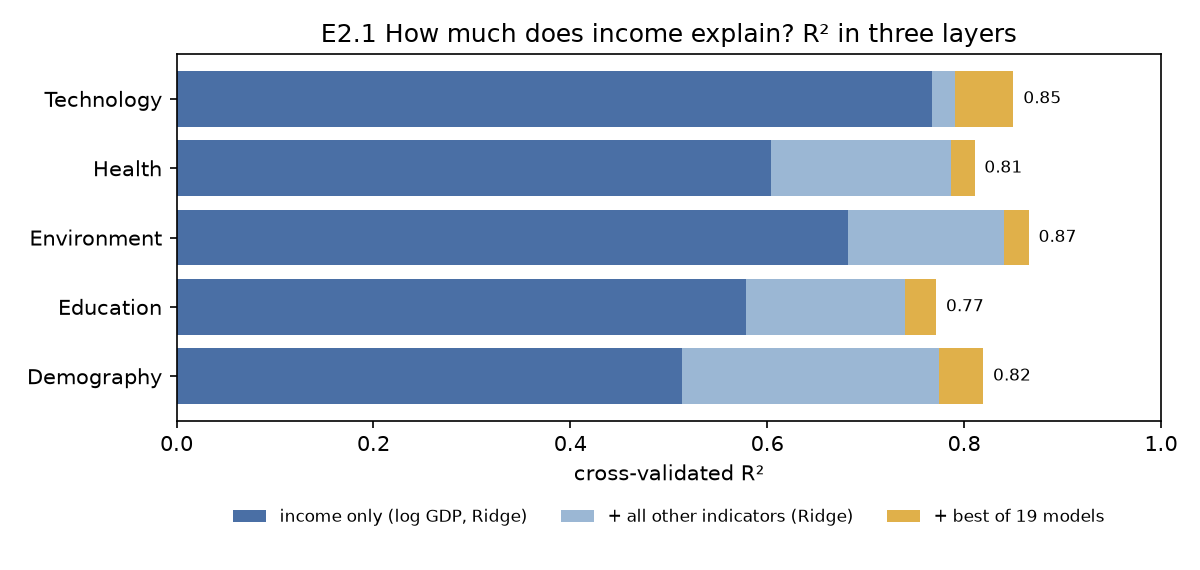
\includegraphics[width=0.95\textwidth]{E2_1_r2_layers.png}
\caption{E2.1: income alone (dark) accounts for most of the explained variance; complex models (yellow) add little.}\label{fig:r2}
\end{figure}
\begin{table}[htbp]\centering
\caption{E2.1: cross-validated $R^2$ (mean $\pm$ SD over five seeds, snapshot, five-fold country-grouped CV).}\label{tab:r2}
\tab{r2}
\end{table}

\paragraph{Performance relative to income (E2.2).} The out-of-fold residual of the income-only model measures how much better or worse a country performs than its income predicts (Figure~\ref{fig:resid}, Table~\ref{tab:resid}). Vietnam has the largest positive life-expectancy residual of all 203 countries (+10.4 years), ranks fourth for internet use (+25 users per 100) and has the third-lowest fertility relative to income ($-1.9$ births per woman). At the same time it emits 3.2 times the CO$_2$ predicted by its income (rank 17 of 199). The largest negative life-expectancy residuals are those of Swaziland, Equatorial Guinea and Angola.

\begin{figure}[htbp]\centering
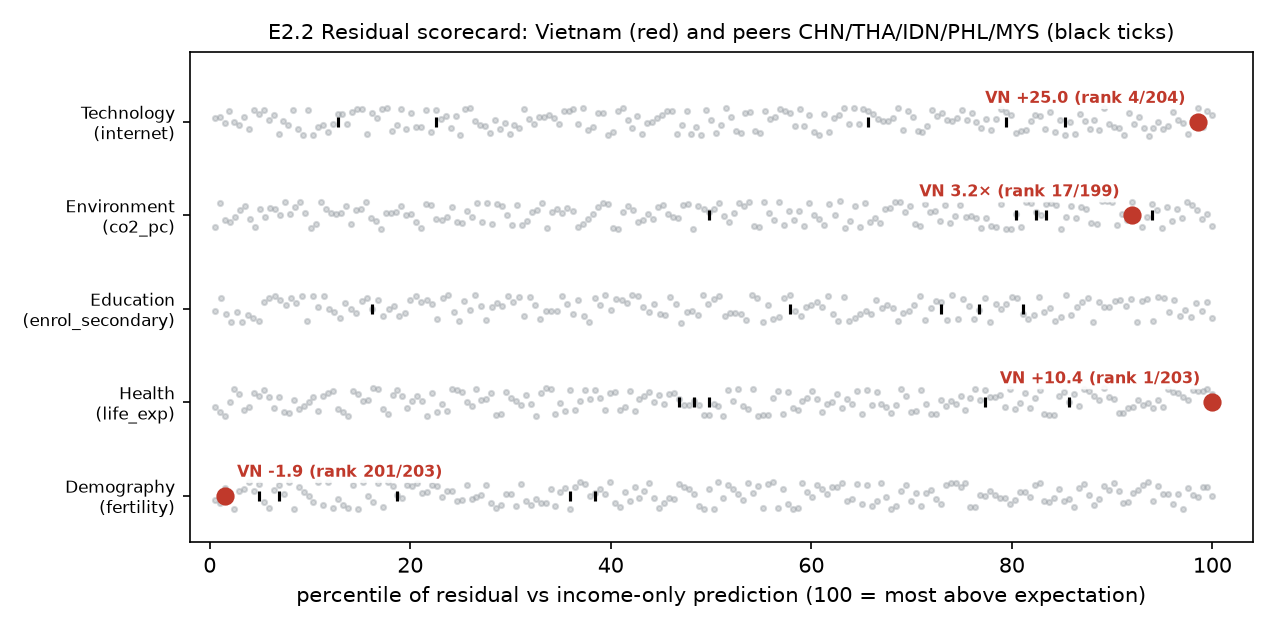
\includegraphics[width=0.9\textwidth]{E2_2_residuals.png}
\caption{E2.2: percentile of each country's residual. Vietnam ranks first of 203 countries for life expectancy and fourth for internet use, and emits 3.2 times its predicted CO$_2$.}\label{fig:resid}
\end{figure}
\begin{table}[htbp]\centering
\caption{E2.2: residuals for Vietnam and its regional comparators (Vietnam does not report secondary enrolment for 2005--2014). For log-transformed targets the residual is the ratio of actual to predicted values.}\label{tab:resid}
\tab{resid}
\end{table}

\paragraph{Within- versus between-country association (E2.3).} The Preston curve compares countries with one another. To assess what happens when a given country becomes richer, the two-way fixed-effects model is estimated (Table~\ref{tab:fe}, Figure~\ref{fig:fe}). A tenfold difference in income between countries is associated with 10.9 additional years of life expectancy, whereas a tenfold increase within a country over time is associated with only 3.2 years (95\,\% CI 1.3--5.2). Most of the gain over time is common to all countries and is captured by the year effects, consistent with diffusion of medical technology and vaccination. This common shift is the reason the Preston curve moved upward by about five years at an income of US\$1,000 and by about four years on average across income levels.

\begin{table}[htbp]\centering
\caption{E2.3: life expectancy regressed on $\log_{10}$ GDP per capita.}\label{tab:fe}
\tab{fe}
\end{table}
\begin{figure}[htbp]\centering
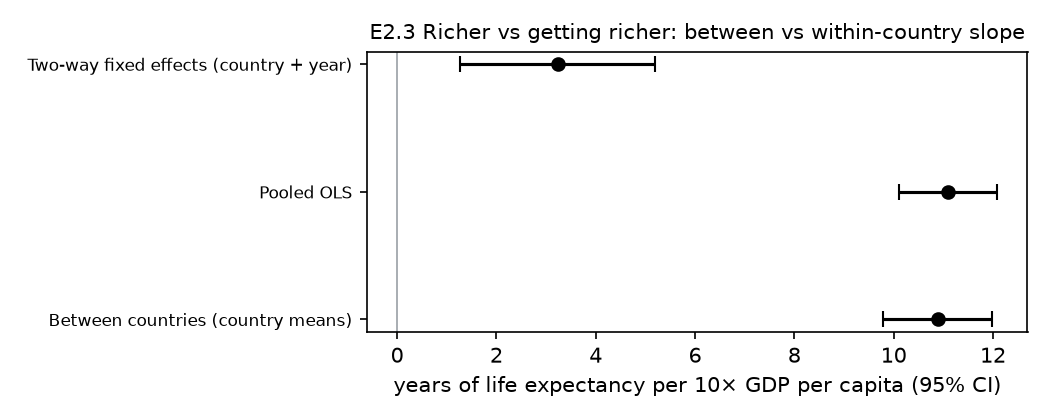
\includegraphics[width=0.9\textwidth]{E2_3_fixed_effects.png}
\caption{E2.3: the within-country slope is approximately one third of the between-country slope.}\label{fig:fe}
\end{figure}

\begin{summary}[Answer to RQ2]
Income alone explains the majority of the cross-country variance in every theme (mean cross-validated $R^2 = 0.63$; H3 supported), and additional model complexity contributes little. The within-country association between income and life expectancy is about one third of the between-country association (H4 supported). The residual identifies countries whose outcomes depart substantially from their income level, with Vietnam showing the largest positive deviation in life expectancy and a substantial negative deviation in carbon intensity.
\end{summary}

\subsection{RQ3: Data-driven groups and the position of Vietnam}

\paragraph{Choice of the number of clusters.} The silhouette coefficient is highest at $k=2$ (0.40) and decreases to 0.19 at $k=4$ (Figure~\ref{fig:k}). The value $k=4$ is retained for interpretability and for comparability with the four income groups.

\begin{figure}[htbp]\centering
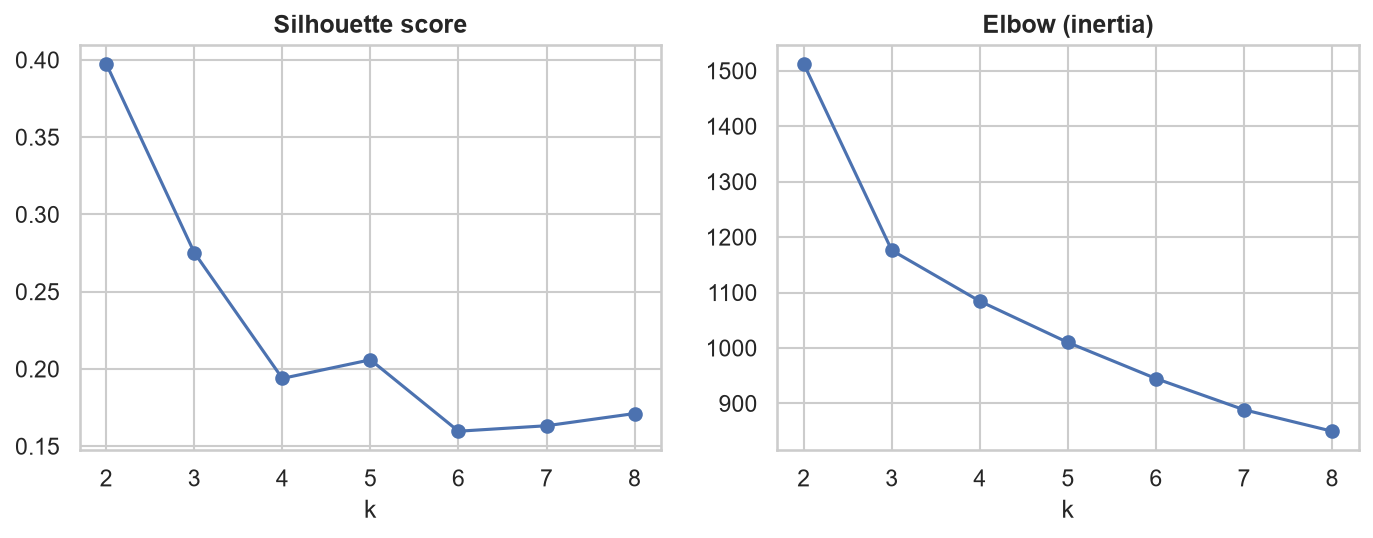
\includegraphics[width=0.85\textwidth]{20_cluster_k.png}
\caption{Choice of $k$: elbow and silhouette criteria. The low silhouette values suggest a continuum rather than well-separated groups.}\label{fig:k}
\end{figure}

\paragraph{Agreement and robustness (E3.1).} K-means is stable across seeds (ARI 0.93) and agrees with the income groups for 74\,\% of countries (Table~\ref{tab:clu}, Figure~\ref{fig:clu}). Across algorithms, however, the partition changes considerably (ARI approximately 0.55), and 77 of the 192 countries remain in the same cluster in fewer than 60\,\% of the 60 runs. The mismatches are informative: oil-rich economies with weak social outcomes, such as Equatorial Guinea and Angola, fall into the low-development cluster. Vietnam is assigned to the emerging cluster in 90\,\% of K-means runs, in 35\,\% of Gaussian-mixture runs and in none of the Ward runs, which places it on the boundary between the transition and emerging clusters.

\begin{table}[htbp]\centering
\caption{E3.1: stability of the partition (reference: K-means with seed 42, as in the web application).}\label{tab:clu}
\tab{clu}
\end{table}
\begin{figure}[htbp]\centering
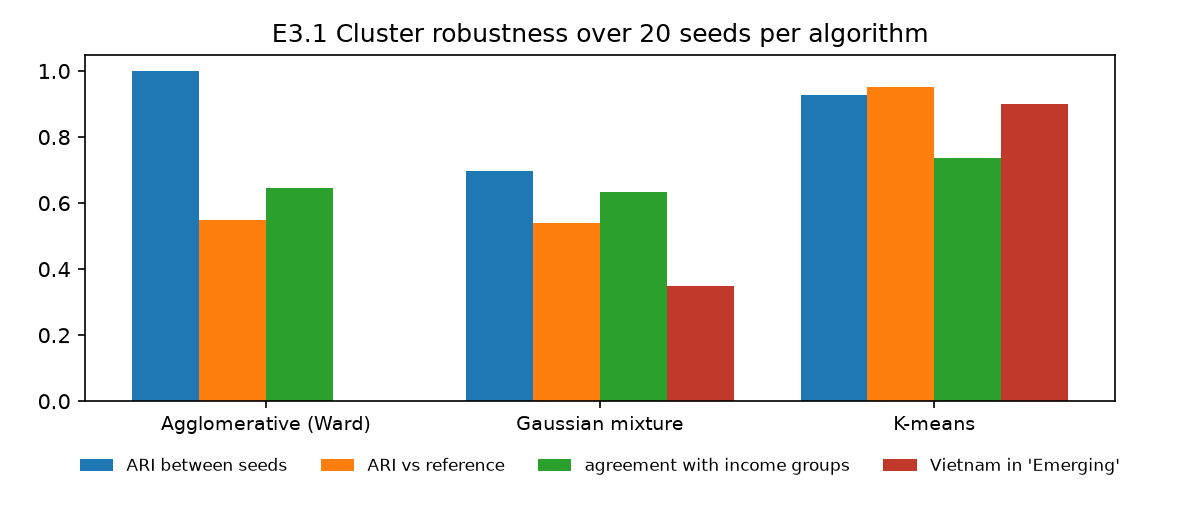
\includegraphics[width=0.95\textwidth]{E3_1_cluster_robustness.png}
\caption{E3.1: K-means is stable across seeds, but the partition depends on the algorithm.}\label{fig:clu}
\end{figure}

\paragraph{Development twins (E3.2).} Measured by income alone, Vietnam's nearest neighbours are Côte d'Ivoire, Nigeria, Zambia, São Tomé and Príncipe and the Solomon Islands, whose life expectancy ranges from 51 to 68 years. Measured by social outcomes, its nearest neighbours are Seychelles, Mauritius and Thailand, which are 3.5 to 14.5 times richer (Table~\ref{tab:twins}). Vietnam's missing secondary-enrolment value is replaced with its income-group median in this distance.

\begin{table}[htbp]\centering
\caption{E3.2: Vietnam's five nearest countries in two feature spaces.}\label{tab:twins}
\tab{twins}
\end{table}

\paragraph{Gap analysis (E3.3).} Relative to the median of the emerging cluster, Vietnam's largest gaps are urbanisation (33\,\% versus 66\,\%, $-1.4$\,SD) and income ($-1.0$\,SD). Under-5 mortality (22 versus 15 per 1,000) constitutes a moderate gap that becomes large ($+1.4$\,SD) relative to the advanced cluster. Vietnam is level with the emerging cluster on health and technology and ahead on trade openness and forest cover (Table~\ref{tab:gaps}, Figure~\ref{fig:gaps}).

\begin{table}[htbp]\centering
\caption{E3.3: Vietnam relative to cluster medians (gap in SD; log scale where indicated). Secondary enrolment is omitted because Vietnam does not report it.}\label{tab:gaps}
\tab{gaps}
\end{table}
\begin{figure}[htbp]\centering
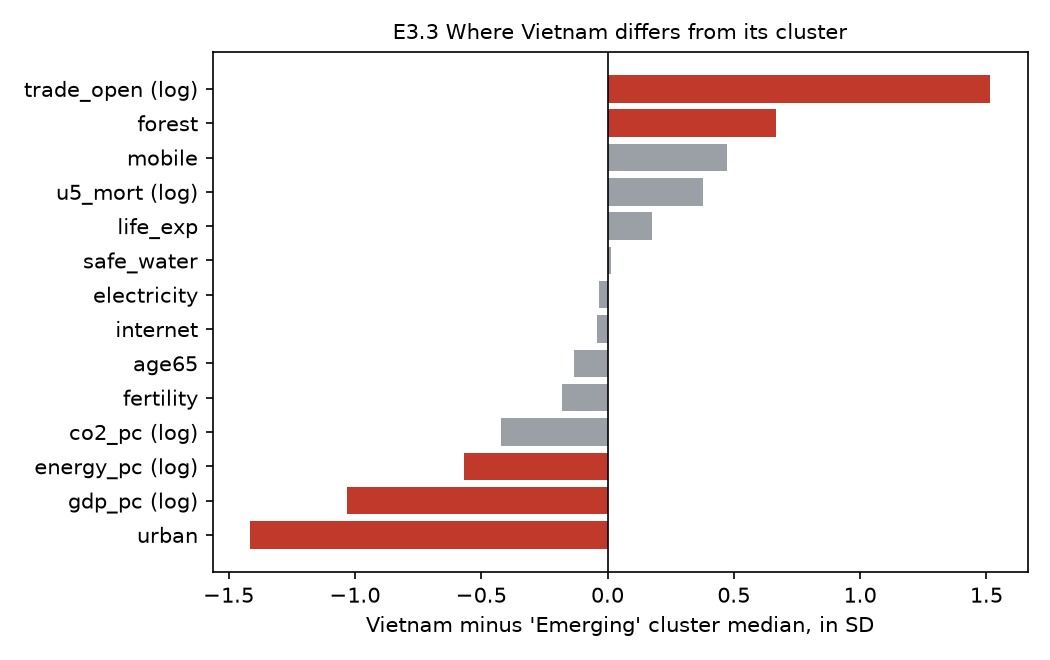
\includegraphics[width=0.9\textwidth]{E3_3_gaps.png}
\caption{E3.3: Vietnam lags the emerging cluster in urbanisation and income, is level in health and technology, and leads in trade openness and forest cover.}\label{fig:gaps}
\end{figure}

\begin{summary}[Answer to RQ3]
Data-driven clusters coincide with the income groups for about three quarters of countries, but the partition is sensitive to the algorithm and cluster separation is weak (H5 partially supported). Development is therefore better described as a continuum along one principal axis. On outcomes, Vietnam resembles countries several times richer; its principal gaps relative to the next group are income, urbanisation and child mortality.
\end{summary}

\subsection{Summary of hypothesis tests}
\begin{table}[htbp]\centering\small
\caption{Summary of the hypothesis tests.}\label{tab:hyp}
\begin{tabular}{p{0.6cm}p{5.4cm}p{6.2cm}p{2.2cm}}
\toprule
& Hypothesis & Evidence & Verdict \\
\midrule
H1 & Social outcomes converged & CV of life expectancy $-47$\,\%, primary enrolment $-67$\,\%, internet $-85$\,\%; robust on balanced panel (E1.1, E1.3) & Supported \\
H2 & Income did not converge & CV of GDP 1.46 $\to$ 1.46; $\beta$-convergence $r=-0.15$, $p=0.054$ (E1.1, E1.2) & Supported \\
H3 & Income explains the majority of variance & income-only $R^2$ 0.51--0.77 (mean 0.63) versus 0.82 for the best model (E2.1) & Supported \\
H4 & Within-country association is weaker & 3.2 versus 10.9 years per tenfold income (E2.3) & Supported \\
H5 & Clusters reproduce income groups & 74\,\% agreement, but ARI $\approx 0.55$ across algorithms and silhouette 0.19 (E3.1) & Partially supported \\
\bottomrule
\end{tabular}
\end{table}

% ================================================================== 7
\section{Interactive web application}\label{sec:app}

\subsection{Purpose and requirements}
The web application serves two purposes: it presents the findings as a self-contained report that can be read without the PDF, and it allows the audience to examine any indicator, country or model interactively during the presentation. The following requirements were defined: (i) every number displayed must be computed from the same data and result files as this report; (ii) the application must run without the 574\,MB raw files; (iii) the structure must follow the assignment (exploration, preprocessing, analysis); and (iv) the interface must remain readable on small screens and in both light and dark modes.

\subsection{Architecture}
The application is implemented in Streamlit and organised as a home page and three further top-level pages, each of which groups its content into tabs (Table~\ref{tab:apppages}). Only the selected tab is computed, which keeps response times short, and each tab has a shareable address (for example \texttt{/findings?tab=why}). Every tab ends with buttons to the previous and next tab in reading order, so the application can be read sequentially like this report. The application reads gzip-compressed copies of the processed tables (\texttt{app\_data/}, 1.5\,MB) and the precomputed result files (\texttt{results/}); it can be started with

\begin{center}\texttt{pip install -r requirements.txt \&\& streamlit run app.py}\end{center}

\begin{table}[htbp]\centering\small
\caption{Pages and tabs of the web application and their correspondence to this report.}\label{tab:apppages}
\begin{tabular}{p{2.0cm}p{3.6cm}p{6.4cm}p{2.4cm}}
\toprule
Page & Tab & Content & Report section \\
\midrule
Home & -- & title, group information, a short summary of the findings (TL;DR), key numbers & Abstract \\
Data & A · Exploration & dataset overview, summary statistics, missing-value impact, outliers, groups & Section~\ref{sec:A} \\
 & B · Preprocessing & problem-to-technique mapping and the result of each technique (B1--B5) & Section~\ref{sec:B} \\
Findings & 1 · What changed & trends, $\sigma$- and $\beta$-convergence, robustness & Section~\ref{sec:conv} \\
 & 2 · Why & income-only fit, residual scorecard, fixed effects & RQ2 \\
 & 3 · So what & PCA, clusters versus income groups, twins, gaps & RQ3 \\
Lab & Trends, Compare, Models, Clusters & free exploration and live re-running of models and clustering & Sections~\ref{sec:method}--\ref{sec:results} \\
\bottomrule
\end{tabular}
\end{table}

The source code separates a shared design and navigation module from one module per page group, so that the three members could develop their parts independently. Results are computed by the \texttt{wdi/} package and consumed by the interface; the clustering pages call the same functions as experiment E3.1, so the application and the report report identical values (for example 74\,\% agreement with the income groups at the default settings).

\subsection{User interface}
Figure~\ref{fig:applanding} shows the home page, Figure~\ref{fig:appdata} the two data tabs, Figure~\ref{fig:appfindings} the three findings tabs and Figure~\ref{fig:applab} two of the laboratory tabs. Each findings section opens with a one-sentence conclusion whose key number is highlighted, followed by the supporting chart; methodological details are available in collapsible panels. All charts are interactive (hover, zoom and legend filtering), and Vietnam is drawn in red throughout.

\begin{figure}[htbp]\centering

\includegraphics[width=0.72\textwidth]{app_report.png}
\caption{Web application: home page with the title, group information and a short summary of the findings.}\label{fig:applanding}
\end{figure}

\begin{figure}[htbp]\centering
\begin{subfigure}{0.49\textwidth}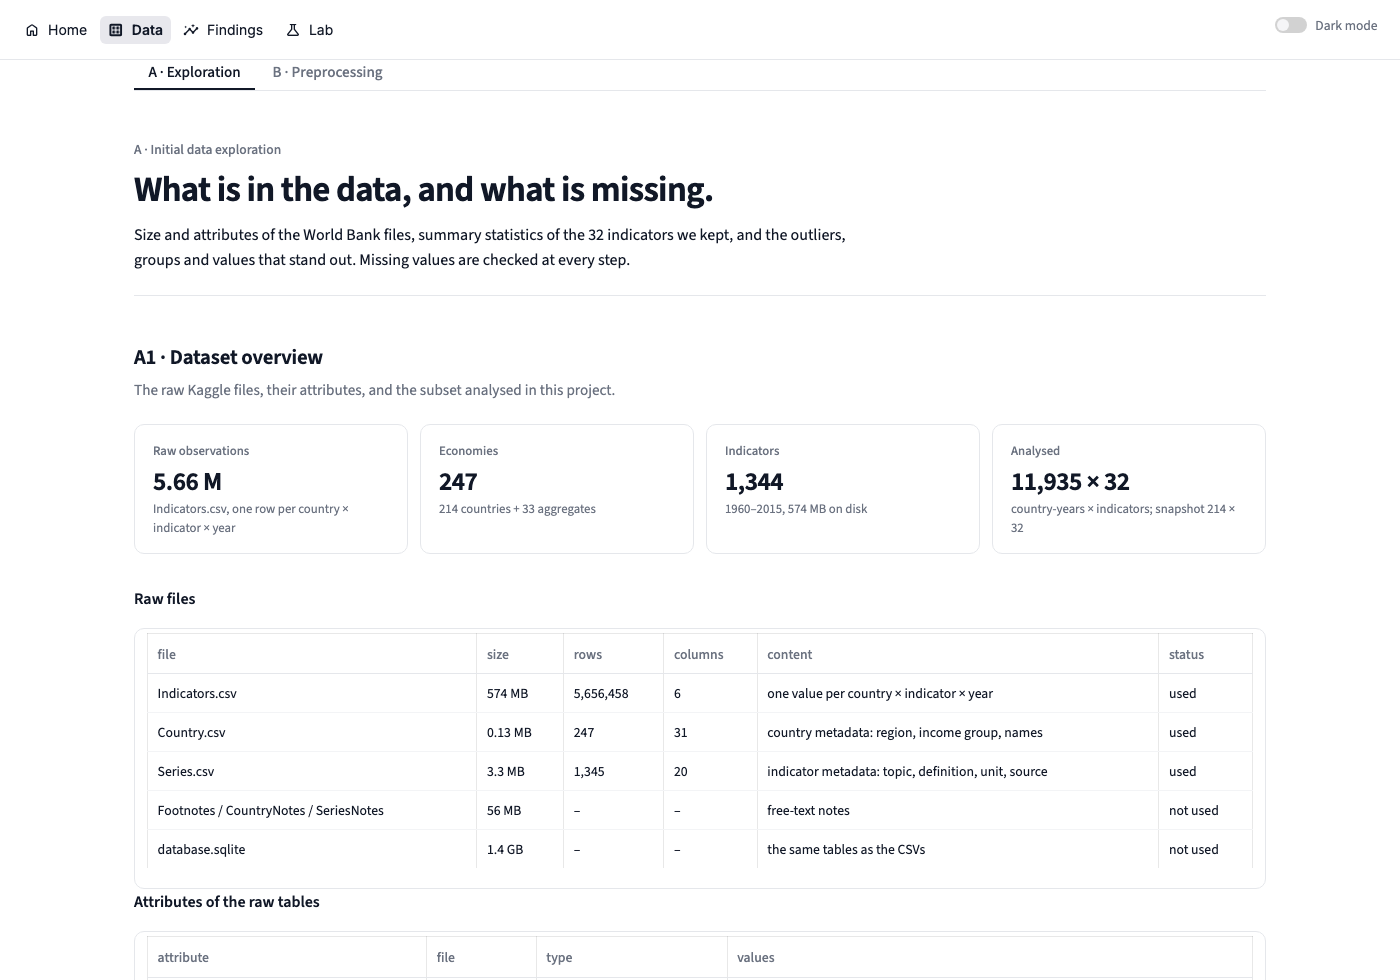
\includegraphics[width=\textwidth]{app_exploration.png}\caption{A · Exploration}\end{subfigure}
\begin{subfigure}{0.49\textwidth}
\includegraphics[width=\textwidth]{app_preprocessing.png}\caption{B · Preprocessing}\end{subfigure}
\caption{Web application: the Data page with its two tabs.}\label{fig:appdata}
\end{figure}

\begin{figure}[htbp]\centering
\begin{subfigure}{0.325\textwidth}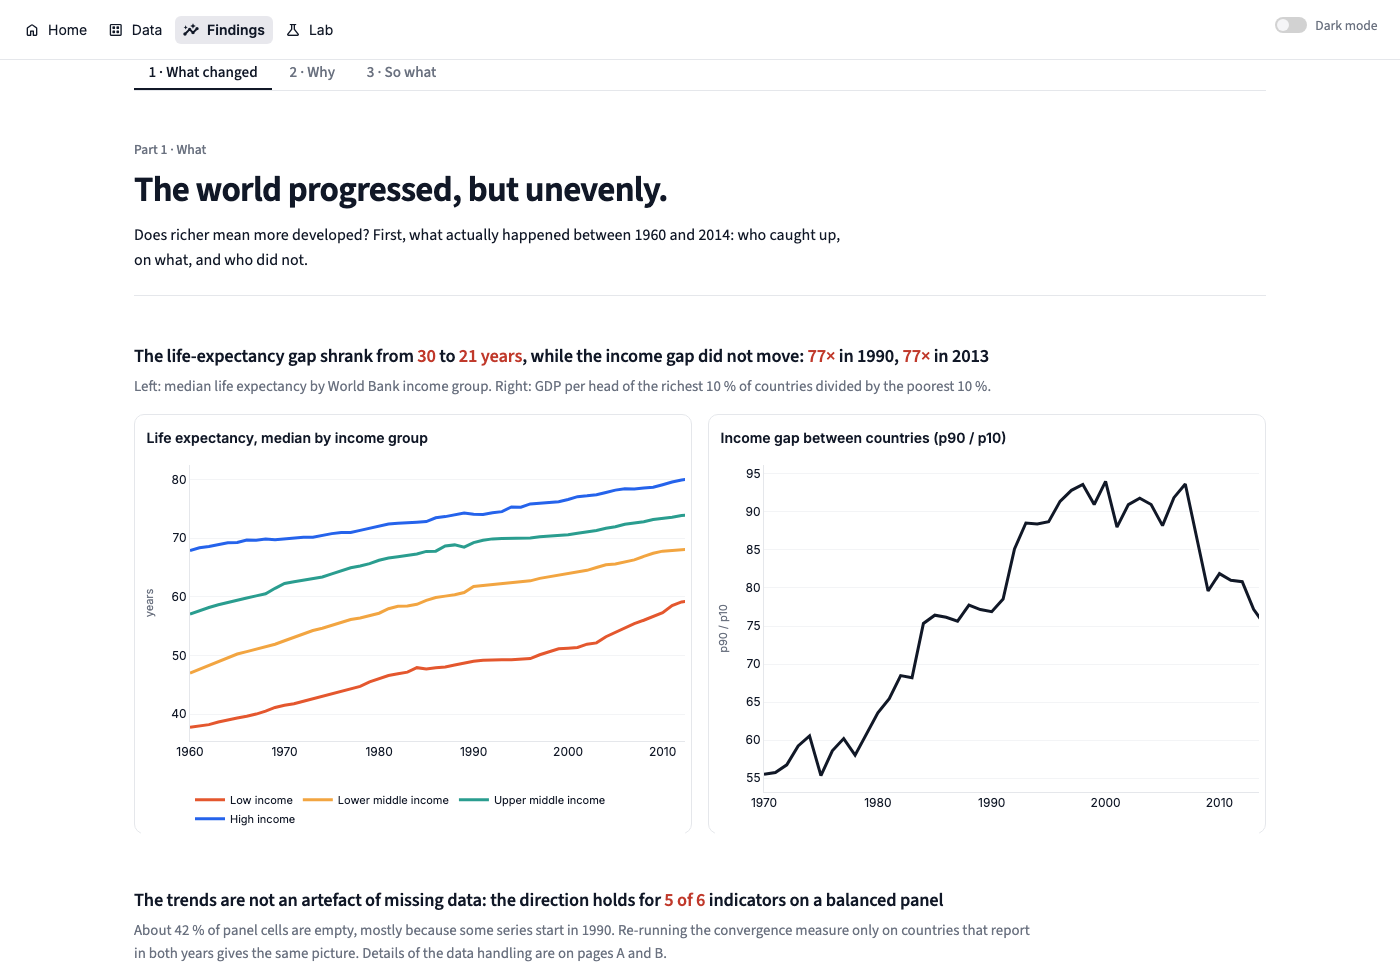
\includegraphics[width=\textwidth]{app_what.png}\caption{1 · What changed}\end{subfigure}
\begin{subfigure}{0.325\textwidth}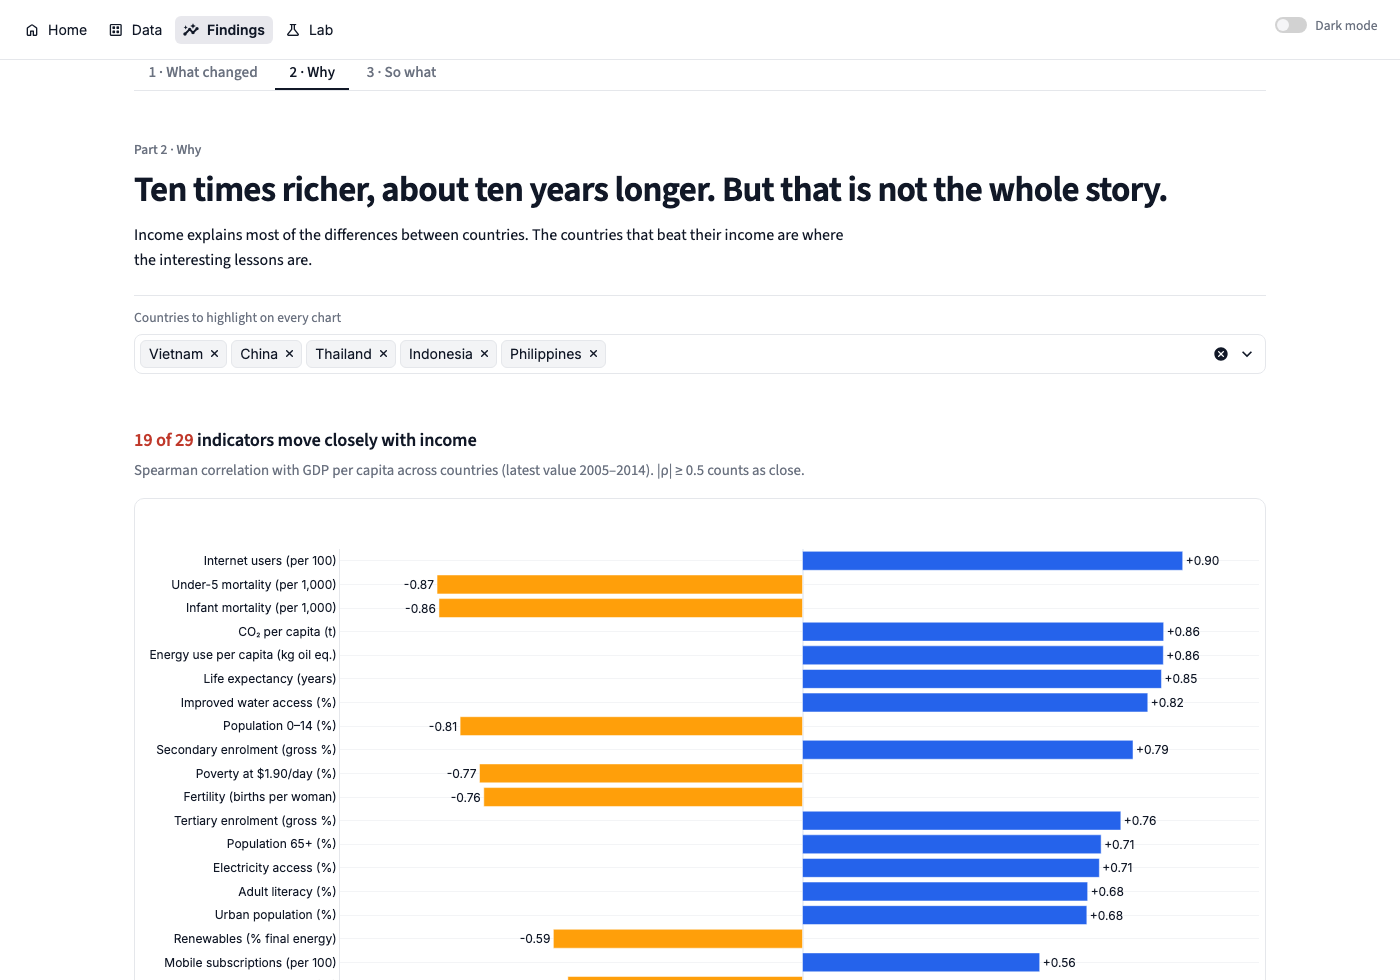
\includegraphics[width=\textwidth]{app_why.png}\caption{2 · Why}\end{subfigure}
\begin{subfigure}{0.325\textwidth}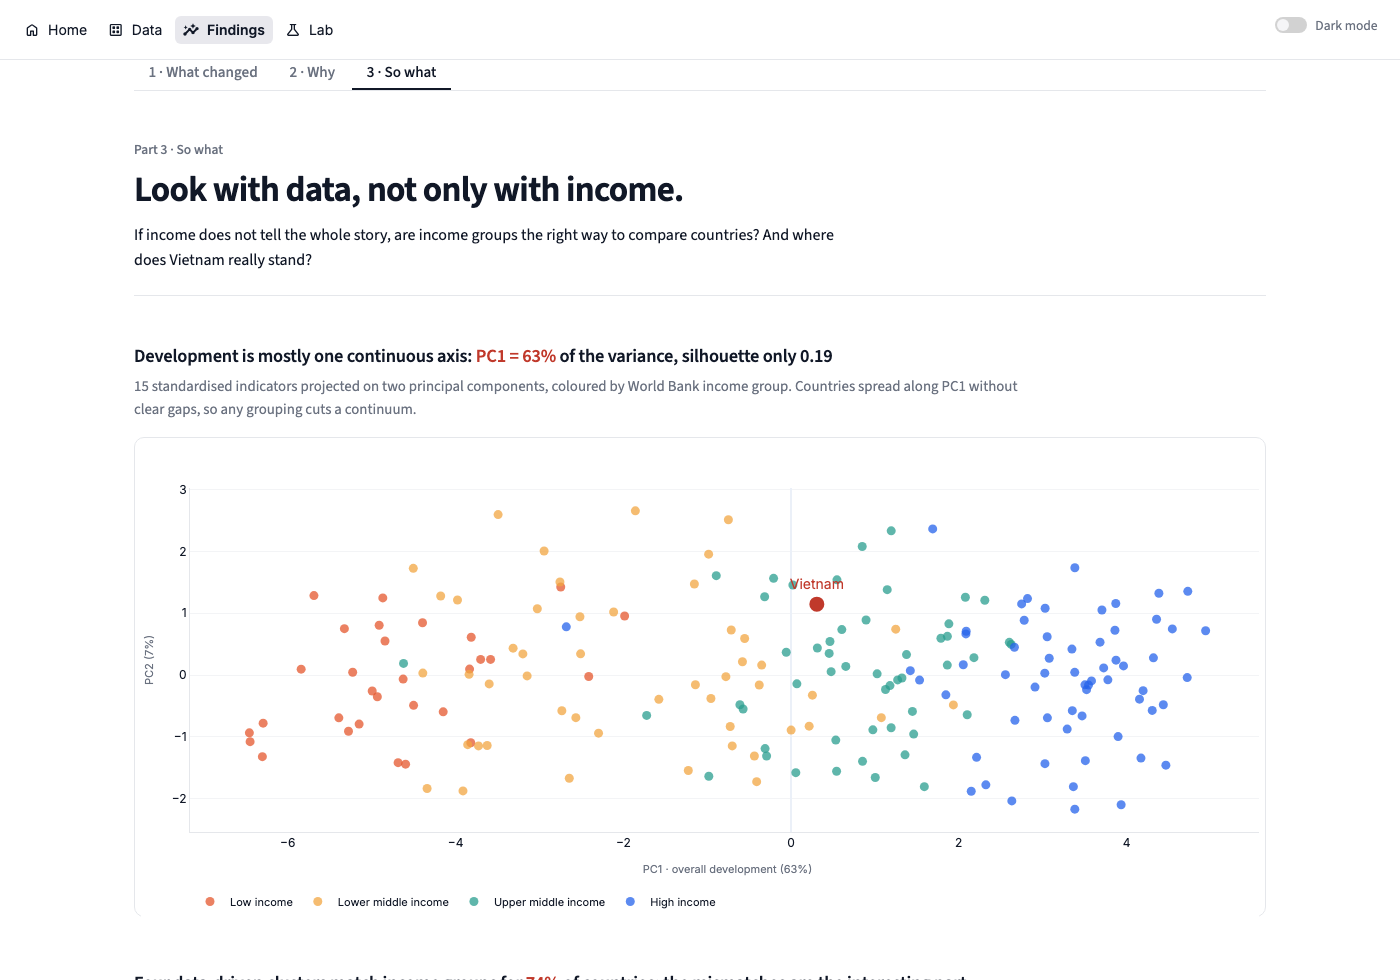
\includegraphics[width=\textwidth]{app_sowhat.png}\caption{3 · So what}\end{subfigure}
\caption{Web application: the Findings page with one tab per research question.}\label{fig:appfindings}
\end{figure}

\begin{figure}[htbp]\centering
\begin{subfigure}{0.49\textwidth}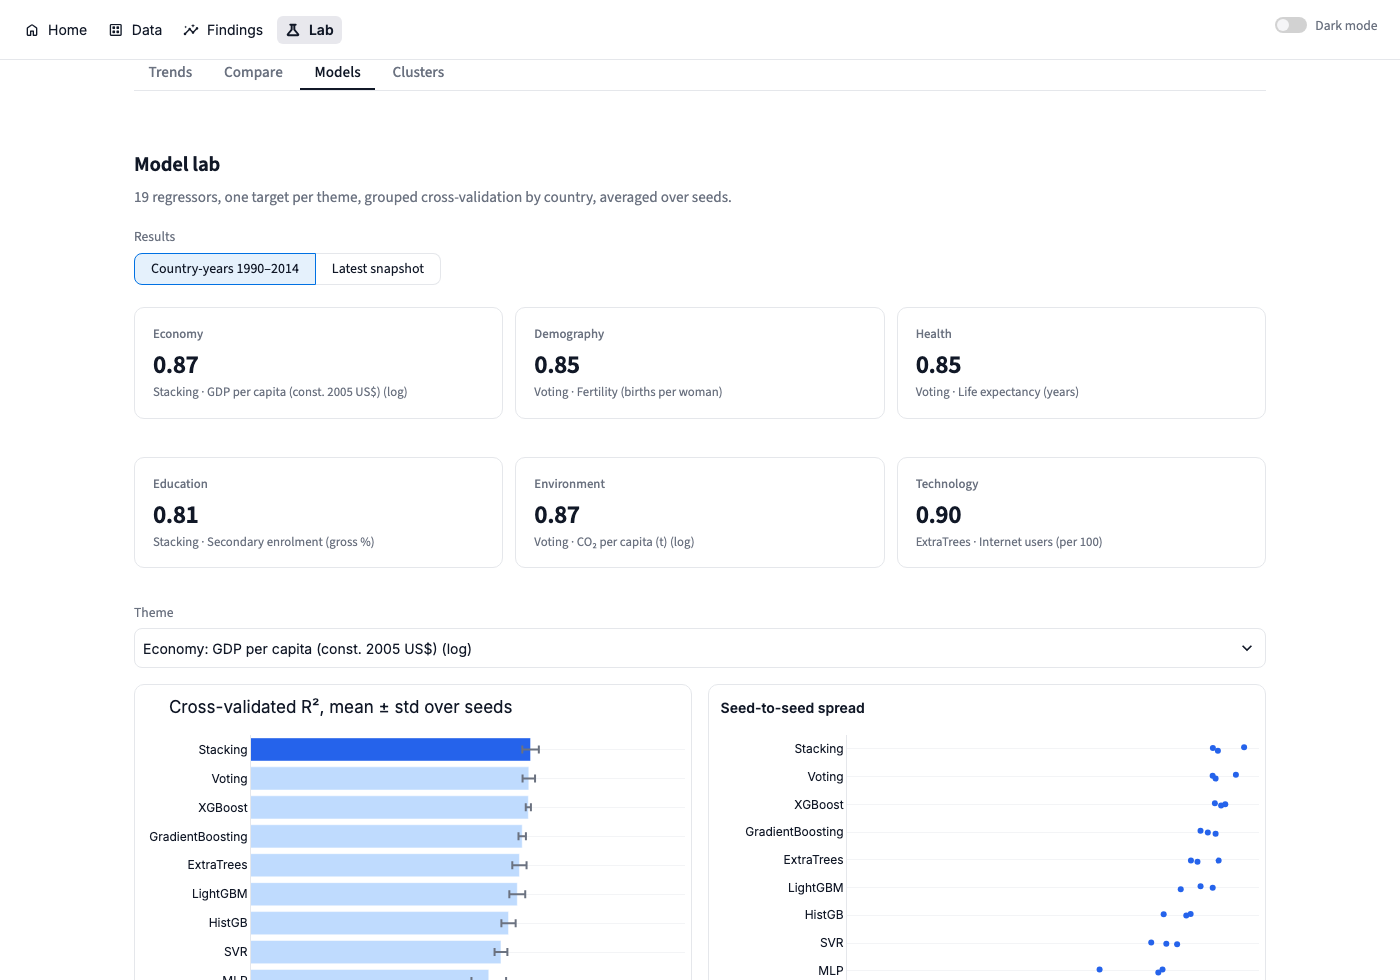
\includegraphics[width=\textwidth]{app_models.png}\caption{Models: $R^2$ of 19 models per theme with seed error bars, permutation importance and live experiments.}\label{fig:appmodels}\end{subfigure}
\begin{subfigure}{0.49\textwidth}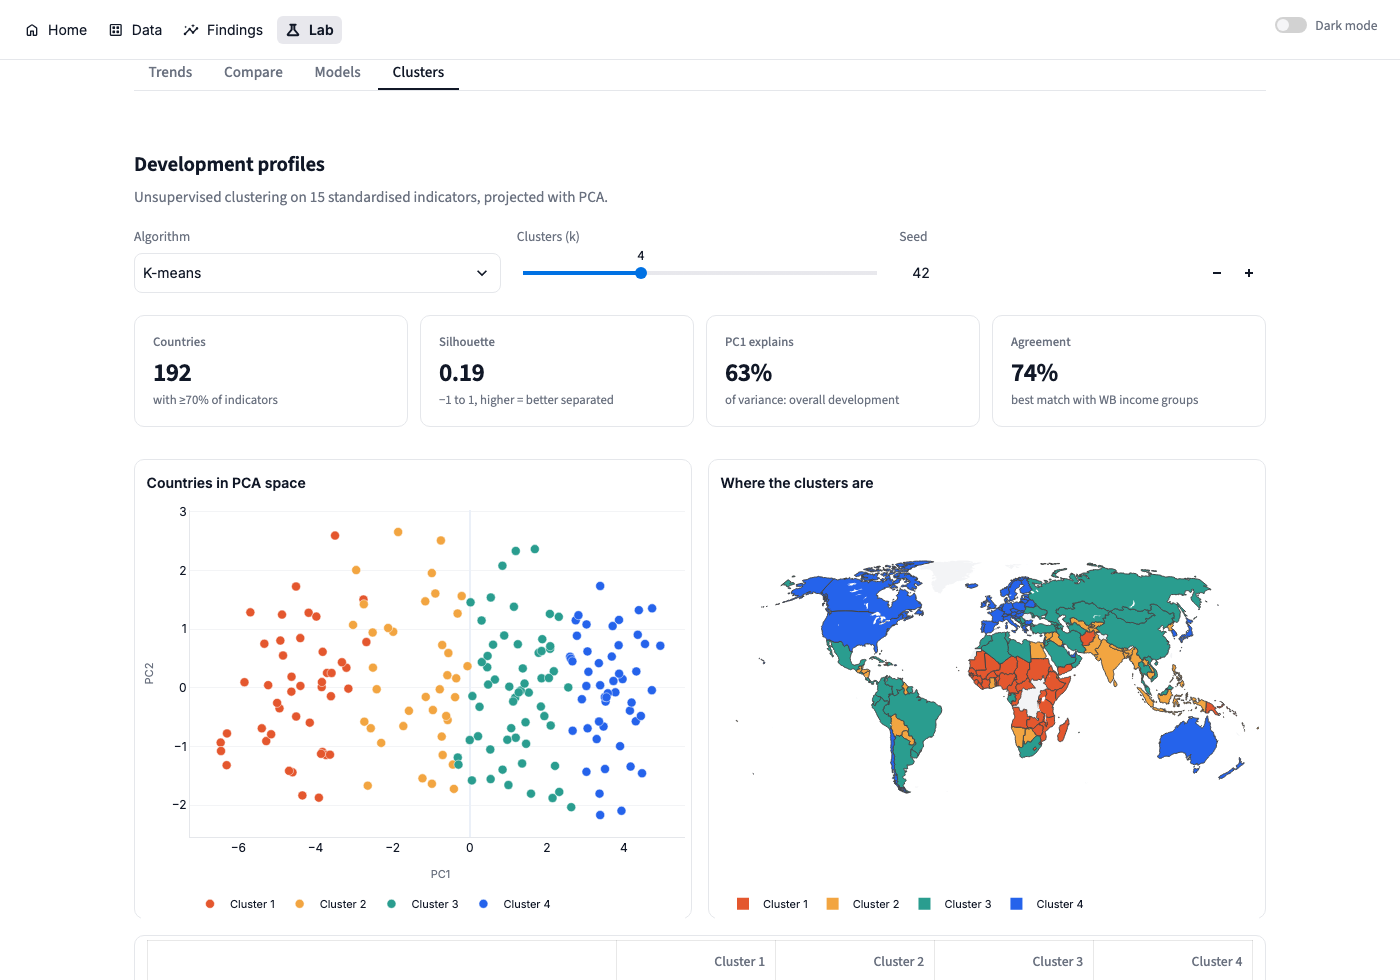
\includegraphics[width=\textwidth]{app_clusters.png}\caption{Clusters: choice of algorithm, $k$ and seed; PCA projection, map and cluster profiles.}\end{subfigure}
\caption{Web application: two tabs of the Lab page.}\label{fig:applab}
\end{figure}

\subsection{Testing}
An automated test renders the home page and each of the nine tabs through its parent page, in both light and dark modes, and fails on any exception or warning; a second test runs the entry point itself. Further tests check that the headline numbers of Sections~\ref{sec:A}--\ref{sec:results} (for example the 29 hyperinflation years, the 69 countries retained under listwise deletion and the PC1 share of 63.5\,\%) are reproduced by the code.

% ================================================================== 8
\section{Discussion}\label{sec:discussion}

\subsection{Principal findings}
The results support a qualified affirmative answer to the overarching question. Higher income is strongly associated with higher development: log GDP per capita alone explains between half and three quarters of the cross-country variance in health, education, demography, environment and technology, and flexible machine-learning models improve on this only marginally. Development indicators are, moreover, so closely interrelated that a single principal component accounts for almost two thirds of their joint variance.

Three findings nevertheless indicate that income is not a sufficient description of development. First, health and schooling converged across countries over five decades while income did not, which implies that social outcomes improved independently of income convergence. Second, the within-country association between income and life expectancy is about one third of the between-country association, and most of the gain over time is common to all countries. Third, the residual from income is large and systematic for a number of countries, and data-driven groupings agree only partially with income groups.

\subsection{Relation to the literature}
The upward shift of the Preston curve and the dominance of year effects in E2.3 are consistent with Preston's interpretation that factors other than income, notably the diffusion of medical knowledge, account for much of the improvement in life expectancy \cite{preston,preston07}. The positive and significant within-country slope is consistent with the finding of Pritchett and Summers \cite{pritchett} that income growth improves health, although the fixed-effects design of this study does not address reverse causality. The large positive residuals of Vietnam and other lower-income countries resemble the low-mortality, low-income cases described by Caldwell \cite{caldwell} and Anand and Ravallion \cite{anand}. The absence of unconditional income convergence agrees with Barro and Sala-i-Martin \cite{barro}, and the concentration of catch-up in a few large economies is consistent with the observation of Sala-i-Martin \cite{sala06} that falling inequality between individuals coexisted with persistent gaps between countries. Finally, the close coupling of CO$_2$ emissions with income ($\rho = 0.86$, comparable to $0.85$ for life expectancy), an estimated environmental Kuznets turning point of about US\$51,000 that only 9 of 192 countries exceed, and the reduction of per-capita emissions in only 26 of 56 high-income countries between 1990 and 2011 provide little support for an environmental Kuznets curve for carbon dioxide within the observed income range \cite{grossman}.

\subsection{Implications}
Two implications follow, both of which should be read as suggestions derived from associations rather than as causal recommendations. First, income-based classifications are a reasonable first approximation, but they conceal substantial heterogeneity; assessments of development benefit from reporting outcomes directly. Second, for Vietnam, the analysis identifies a strong position in health and technology relative to income, together with comparatively low urbanisation, a remaining gap in child mortality relative to advanced economies, and a carbon intensity well above its income level. Sustaining the social advantage while following a less carbon-intensive growth path than earlier industrialisers appears to be the principal challenge indicated by the data.

\subsection{Threats to validity}\label{sec:validity}
\begin{itemize}
\item \emph{Data currency.} The extract ends in 2014--2015 (CO$_2$ in 2011) and uses the income classification and 2005 price base of that time; more recent developments are not captured.
\item \emph{Missing data not at random.} Poorer countries report less often, and high-income countries do not report extreme poverty. Interpolation, the snapshot window, in-fold imputation and the robustness checks of E1.3 mitigate but do not eliminate the resulting bias for survey indicators.
\item \emph{Association, not causation.} The fixed-effects model removes time-invariant country characteristics and common shocks but does not identify a causal effect of income; time-varying confounders and reverse causality remain possible.
\item \emph{Unweighted country medians.} Each country has equal weight, so small states count as much as China or India. E1.3 shows that population weighting does not alter the direction of the convergence results.
\item \emph{Territorial emissions.} CO$_2$ is measured on a production basis and ignores emissions embodied in trade.
\item \emph{Cluster validity.} Silhouette values are low and partitions depend on the algorithm, so cluster labels should be interpreted as positions on a continuum rather than as natural groups.
\end{itemize}

% ================================================================== 9
\section{Conclusion and future work}\label{sec:conclusion}
This study examined, on 32 World Development Indicators for 214 countries over 1960--2014, whether higher national income corresponds to higher development. After a systematic exploration of the data and a preprocessing pipeline designed around the problems identified, nine experiments addressed three research questions. The results show that income alone explains the majority of the cross-country variation in development outcomes (mean cross-validated $R^2 = 0.63$), and that more complex models add little to this. Income, however, is not a sufficient description of development: health and schooling converged across countries while income did not, the association within countries over time is about one third of that between countries, and data-driven groupings agree with income groups for only about three quarters of countries. Vietnam illustrates the limits of an income-based view, combining social outcomes typical of much richer countries with a carbon intensity well above its income level.

Future work could (i) extend the analysis to the 2020s with data from the live WDI interface, (ii) apply dynamic panel and instrumental-variable methods to approach causal questions, (iii) repeat the convergence and clustering analyses with population weights and consumption-based CO$_2$ accounting, and (iv) investigate the policy characteristics of the countries with the largest positive residuals.

\begin{thebibliography}{99}\addcontentsline{toc}{section}{References}
\bibitem{wdi} World Bank (2016). \emph{World Development Indicators}. Washington, DC: The World Bank. \url{https://datatopics.worldbank.org/world-development-indicators/}
\bibitem{kaggle} Kaggle / World Bank (2017). \emph{World Development Indicators} dataset. \url{https://www.kaggle.com/datasets/kaggle/world-development-indicators}
\bibitem{preston} Preston, S.~H. (1975). The changing relation between mortality and level of economic development. \emph{Population Studies}, 29(2), 231--248.
\bibitem{preston07} Preston, S.~H. (2007). The changing relation between mortality and level of economic development. \emph{International Journal of Epidemiology}, 36(3), 484--490.
\bibitem{bloom07} Bloom, D.~E. and Canning, D. (2007). Commentary: The Preston Curve 30 years on: still sparking fires. \emph{International Journal of Epidemiology}, 36(3), 498--499.
\bibitem{pritchett} Pritchett, L. and Summers, L.~H. (1996). Wealthier is healthier. \emph{Journal of Human Resources}, 31(4), 841--868.
\bibitem{deaton} Deaton, A. (2003). Health, inequality, and economic development. \emph{Journal of Economic Literature}, 41(1), 113--158.
\bibitem{caldwell} Caldwell, J.~C. (1986). Routes to low mortality in poor countries. \emph{Population and Development Review}, 12(2), 171--220.
\bibitem{anand} Anand, S. and Ravallion, M. (1993). Human development in poor countries: on the role of private incomes and public services. \emph{Journal of Economic Perspectives}, 7(1), 133--150.
\bibitem{mrw} Mankiw, N.~G., Romer, D. and Weil, D.~N. (1992). A contribution to the empirics of economic growth. \emph{Quarterly Journal of Economics}, 107(2), 407--437.
\bibitem{sala06} Sala-i-Martin, X. (2006). The world distribution of income: falling poverty and \ldots\ convergence, period. \emph{Quarterly Journal of Economics}, 121(2), 351--397.
\bibitem{barro} Barro, R.~J. and Sala-i-Martin, X. (1992). Convergence. \emph{Journal of Political Economy}, 100(2), 223--251.
\bibitem{grossman} Grossman, G.~M. and Krueger, A.~B. (1995). Economic growth and the environment. \emph{Quarterly Journal of Economics}, 110(2), 353--377.
\bibitem{little} Little, R.~J.~A. and Rubin, D.~B. (2019). \emph{Statistical Analysis with Missing Data} (3rd ed.). Wiley.
\bibitem{han} Han, J., Kamber, M. and Pei, J. (2011). \emph{Data Mining: Concepts and Techniques} (3rd ed.). Morgan Kaufmann.
\bibitem{wooldridge} Wooldridge, J.~M. (2010). \emph{Econometric Analysis of Cross Section and Panel Data} (2nd ed.). MIT Press.
\bibitem{rousseeuw} Rousseeuw, P.~J. (1987). Silhouettes: a graphical aid to the interpretation and validation of cluster analysis. \emph{Journal of Computational and Applied Mathematics}, 20, 53--65.
\bibitem{hubert} Hubert, L. and Arabie, P. (1985). Comparing partitions. \emph{Journal of Classification}, 2(1), 193--218.
\bibitem{breiman} Breiman, L. (2001). Random forests. \emph{Machine Learning}, 45(1), 5--32.
\bibitem{xgb} Chen, T. and Guestrin, C. (2016). XGBoost: a scalable tree boosting system. In \emph{Proc.\ KDD 2016}, 785--794.
\bibitem{lgbm} Ke, G. et al.\ (2017). LightGBM: a highly efficient gradient boosting decision tree. In \emph{Advances in Neural Information Processing Systems 30}.
\bibitem{sklearn} Pedregosa, F. et al.\ (2011). Scikit-learn: machine learning in Python. \emph{Journal of Machine Learning Research}, 12, 2825--2830.
\bibitem{pandas} McKinney, W. (2010). Data structures for statistical computing in Python. In \emph{Proc.\ 9th Python in Science Conference}, 56--61.
\bibitem{streamlit} Streamlit (2024). \emph{Streamlit documentation}. \url{https://docs.streamlit.io}
\end{thebibliography}

% ================================================================== appendix
\appendix
\section{Selected indicators}\label{app:vars}
\begin{table}[htbp]\centering\footnotesize
\caption{The 32 selected indicators.}\label{tab:vars}
\begin{adjustbox}{max width=\textwidth}\begin{tabular}{lll|lll}
\toprule
Alias & WDI code & Theme & Alias & WDI code & Theme \\
\midrule
\var{gdp\_pc} & NY.GDP.PCAP.KD & Economy & \var{infant\_mort} & SP.DYN.IMRT.IN & Health \\
\var{gdp\_pc\_ppp} & NY.GDP.PCAP.PP.KD & Economy & \var{u5\_mort} & SH.DYN.MORT & Health \\
\var{gdp\_growth} & NY.GDP.MKTP.KD.ZG & Economy & \var{health\_exp} & SH.XPD.TOTL.ZS & Health \\
\var{inflation} & FP.CPI.TOTL.ZG & Economy & \var{safe\_water} & SH.H2O.SAFE.ZS & Health \\
\var{unemployment} & SL.UEM.TOTL.ZS & Economy & \var{enrol\_primary} & SE.PRM.ENRR & Education \\
\var{trade\_open} & NE.TRD.GNFS.ZS & Economy & \var{enrol\_secondary} & SE.SEC.ENRR & Education \\
\var{gini} & SI.POV.GINI & Economy & \var{enrol\_tertiary} & SE.TER.ENRR & Education \\
\var{poverty\_190} & SI.POV.DDAY & Economy & \var{literacy} & SE.ADT.LITR.ZS & Education \\
\var{population} & SP.POP.TOTL & Demography & \var{edu\_exp} & SE.XPD.TOTL.GD.ZS & Education \\
\var{pop\_growth} & SP.POP.GROW & Demography & \var{co2\_pc} & EN.ATM.CO2E.PC & Environment \\
\var{urban} & SP.URB.TOTL.IN.ZS & Demography & \var{energy\_pc} & EG.USE.PCAP.KG.OE & Environment \\
\var{fertility} & SP.DYN.TFRT.IN & Demography & \var{forest} & AG.LND.FRST.ZS & Environment \\
\var{age65} & SP.POP.65UP.TO.ZS & Demography & \var{renewables} & EG.FEC.RNEW.ZS & Environment \\
\var{age0\_14} & SP.POP.0014.TO.ZS & Demography & \var{electricity} & EG.ELC.ACCS.ZS & Technology \\
\var{female\_lfp} & SL.TLF.CACT.FE.ZS & Demography & \var{internet} & IT.NET.USER.P2 & Technology \\
\var{life\_exp} & SP.DYN.LE00.IN & Health & \var{mobile} & IT.CEL.SETS.P2 & Technology \\
\bottomrule
\end{tabular}\end{adjustbox}
\end{table}

\section{Repository structure}\label{app:repo}
\begin{adjustbox}{max width=\textwidth}\begin{tabular}{ll}
\toprule
Path & Content \\
\midrule
\texttt{Makefile} & one command per stage of the pipeline (\texttt{make all} reproduces every result, \texttt{make app} starts the application) \\
\texttt{WDI\_Analysis.ipynb} & ETL, missing-data audit, exploratory analysis, trends, comparisons, evaluation \\
\texttt{wdi/models.py}, \texttt{run\_models.py} & suite of 19 models with country-grouped cross-validation \\
\texttt{wdi/story/}, \texttt{run\_story.py} & exploration and preprocessing checks (A, B) and experiments E1.1--E3.3 \\
\texttt{app.py}, \texttt{ui/} & Streamlit web application (Home, Data, Findings, Lab) \\
\texttt{app\_data/} & compressed processed tables, so that the application runs without the raw files \\
\texttt{results/}, \texttt{results/story/} & model and experiment results (CSV) \\
\texttt{figures/} & figures used in this report \\
\texttt{report/} & this report and the scripts that generate its tables and figures \\
\texttt{tests/} & automated tests of the models, experiments and web application \\
\bottomrule
\end{tabular}\end{adjustbox}

\end{document}
